\documentclass[%
%draft,
11pt,%
twoside,%
titlepage,%
swissgerman,%
headsepline%
]{scrartcl}

\usepackage{lastpage}
\usepackage{amsthm}
\usepackage{amssymb}
\usepackage{geometry}
\usepackage{graphicx}
\usepackage[dvipsnames]{xcolor}
\usepackage[utf8]{inputenc}
\usepackage[swissgerman]{babel}
\usepackage{lscape}
\usepackage[framemethod=TikZ]{mdframed}
\usepackage[most]{tcolorbox}
\usepackage{enumerate}
\usepackage{units}
\usepackage{nicefrac}
\usepackage{pgf,tikz}
\usepackage{tikz-3dplot}
\usepackage{tkz-euclide}
\usetikzlibrary{arrows}
\usetikzlibrary{arrows.meta}
\usetikzlibrary{patterns}
\usetikzlibrary{positioning}
\usetikzlibrary{shadows}
\usetikzlibrary{quotes, angles}
\usepackage{colortbl}
\usepackage{hhline}
\usepackage{multirow}
\usepackage[extendedchars]{grffile}
\usepackage{caption}
\usepackage{multicol,calc}
\usepackage{blindtext}
\usepackage{pdfpages}
\usepackage{hyperref}
\usepackage{framed}

\usepackage{marginnote}
\usepackage{qrcode}
\qrset{height=9ex}

\usepackage{longtable}
\usepackage{listings}
\usepackage{wrapfig}

\usepackage{fontawesome} % Oder FontAwesome, falls du ein Augensymbol aus einer
\newcommand{\faEyeLightGray}{\textcolor{lightgray}{\faEye}} % Custom command for the gray eye icon
\newcommand{\faReturnGray}{\textcolor{gray}{\faMailReply}} % Custom command for the gray eye icon
\usepackage{pifont} % weitere Zeichen

% package für plots mit dem Befehl axes
\usepackage{pgfplots}



% Command, um Tabellen-Spalten anzupassen
\newcommand{\spaltenheight}{\rule{0mm}{3ex}}
\newcommand{\spaltenwidth}{\rule{3cm}{0mm}}
\newcommand{\spaltensep}{\\[1ex]}
%\arrayrulecolor{darkgreen}
\doublerulesepcolor{white}

% colors
\definecolor{lightyellow}{rgb}{1,1,0.8}
\definecolor{Gray}{gray}{0.9}
\definecolor{lightgray}{rgb}{0.7, 0.7, 0.7}
\definecolor{darkblue}{rgb}{0,0,0.55}
\definecolor{firebrick}{rgb}{0.7,0.13,0.13}
\definecolor{seagreen}{rgb}{0.18,0.55,0.34}
\definecolor{emerald}{HTML}{50C878} % color of Definition
\definecolor{whitesmoke}{HTML}{F5F5F5} % background for environments
\definecolor{myblizzardblue}{HTML}{87CEEB} % color of Satz

% Für Definitionen im Fliesstext
\newcommand{\definition}[1]{\colorbox{emerald}{#1}}
% Für Regeln im Fliesstext
\newcommand{\regel}[1]{\colorbox{myblizzardblue}{#1}}
% Für Merke/Achtungs im Fliesstext
\newcommand{\merke}[1]{\colorbox{firebrick}{#1}}
% Geogebra-Link
\newcommand{\geogebralink}{\href{https://www.geogebra.org/calculator}{\texttt{geogebra.org}}}

% Umgebungen
\theoremstyle{definition}
    \newtheorem{bsp}{Beispiel}[subsection] % Beispiele
    \newtheorem{bem}{Bemerkung}[subsection] % Bemerkungen
\theoremstyle{plain}
    \newtheorem{thm}{Theorem} % Theorem [subsection]
    \newtheorem{satz}{Satz} % Satz [subsection]

% Umgebung lsg mit dynamischer Referenzierung und Label
\newcommand{\concatueb}[1]{ueb:#1}% Definition für concatueb
\newcommand{\concatlsg}[1]{lsg:#1}% Definition für concatlsg

\newcounter{uebcounter}[section]
\renewcommand{\theuebcounter}{\thesection.\arabic{uebcounter}}  % Zählerformat: Abschnitt.Übung

\newenvironment{lsg}[1]{%
    \par\noindent\textbf{Notizen zu Übung \theuebcounter\label{\concatlsg{#1}}}
    \hfill\hyperref[\concatueb{#1}]{\faReturnGray}\par % Hyperref-Button zurück zur Übung
}{%
    \par%
}

\newenvironment{uebenv}[1]{%
    \refstepcounter{uebcounter}
    \par\noindent\textbf{Übung \theuebcounter.}%
    \label{\concatueb{#1}}\hfill\hyperref[\concatlsg{#1}]{\faEyeLightGray}\par
}{%
    \par
}

% Umgebung für Definitionen
\newcounter{deff}[section]\setcounter{deff}{0}
\renewcommand{\thedeff}{\arabic{section}.\arabic{deff}}

\newenvironment{cdef}[1][]{%
    \refstepcounter{deff} 
    \ifstrempty{#1}%
    % if condition (without title)
    {\mdfsetup{%
        frametitle={%
            \tikz[baseline=(current bounding box.east),outer sep=0pt]
            \node[anchor=east,rectangle,fill=emerald]
            {\strut Definition~\thedeff};}
        }%
    % else condition (with title)
    }{\mdfsetup{%
        frametitle={%
            \tikz[baseline=(current bounding box.east),outer sep=0pt]
            \node[anchor=east,rectangle,fill=emerald]
            {\strut Definition~\thedeff:~#1};}%
        }%
    }%
% for both conditions
    \mdfsetup{%
        innertopmargin=10pt,linecolor=emerald,%
        backgroundcolor=whitesmoke,%
        linewidth=2pt,topline=true,%
        frametitleaboveskip=\dimexpr-\ht\strutbox\relax%
    } 
\begin{mdframed}[]\relax}{%
\end{mdframed}}

% Farbig umrahmte Umgebung Satz
\newcounter{satzz}[section]\setcounter{satzz}{0}
\renewcommand{\thesatz}{\arabic{section}.\arabic{satzz}}

\newenvironment{csatz}[1][]{%
    \refstepcounter{satzz}
 
    \ifstrempty{#1}%
    % if condition (without title)
    {\mdfsetup{%
        frametitle={%
            \tikz[baseline=(current bounding box.east),outer sep=0pt]
            \node[anchor=east,rectangle,fill=myblizzardblue]
            {\strut Satz~\thesatz};}
        }%
    % else condition (with title)
    }{\mdfsetup{%
        frametitle={%
            \tikz[baseline=(current bounding box.east),outer sep=0pt]
            \node[anchor=east,rectangle,fill=myblizzardblue]
            {\strut Satz~\thesatz:~#1};}%
        }%
    }%
% for both conditions
    \mdfsetup{%
        innertopmargin=10pt,linecolor=myblizzardblue,%
        backgroundcolor=whitesmoke,%
        linewidth=2pt,topline=true,%
        frametitleaboveskip=\dimexpr-\ht\strutbox\relax%
    }
\begin{mdframed}[]\relax}{%
\end{mdframed}}

% kein Einzug bei neuem Abschnitt
\setlength{\parindent}{0pt} \setlength{\parskip}{1em}
\pagestyle{headings} % gemachte Einstellungen anwenden

\subject{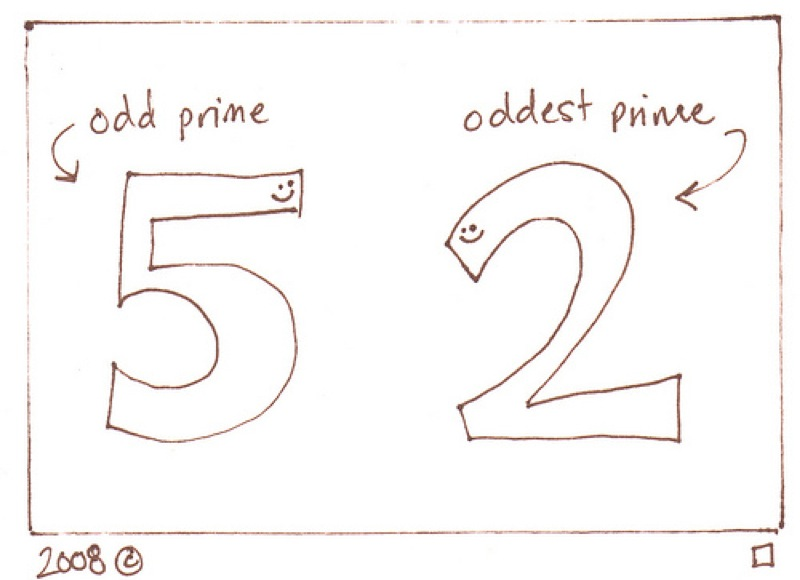
\includegraphics[width=0.618\textwidth]{pictures/primzahl.jpeg}}
\title{Zahlen \& Rechnen}
\subtitle{I like $\mathbb{P}$}
\author{}
\date{}
\lowertitleback{

\includegraphics[height=1cm]{pictures/gymfmslerbermattlogo.eps}
\hfill%\copyright%
{\begin{tikzpicture}
  % Draw the rounded rectangle and clip the image to it
  \clip [rounded corners=5mm] (0,0) rectangle (1,1); % Adjust dimensions as needed
  \node at (0.5,0.5) {\includegraphics[width=1cm]{pictures/teacher_me_caricatur.png}}; % Adjust width and center image
\end{tikzpicture}}
}

\begin{document}
\maketitle
\tableofcontents
%\thispagestyle{empty}
\cleardoublepage
%\setcounter{page}{1}


\section{Mengenlehre}

\subsection{Historisches zur Mengenlehre}
\begin{wrapfigure}{r}{0.382\textwidth}
  \begin{center}
    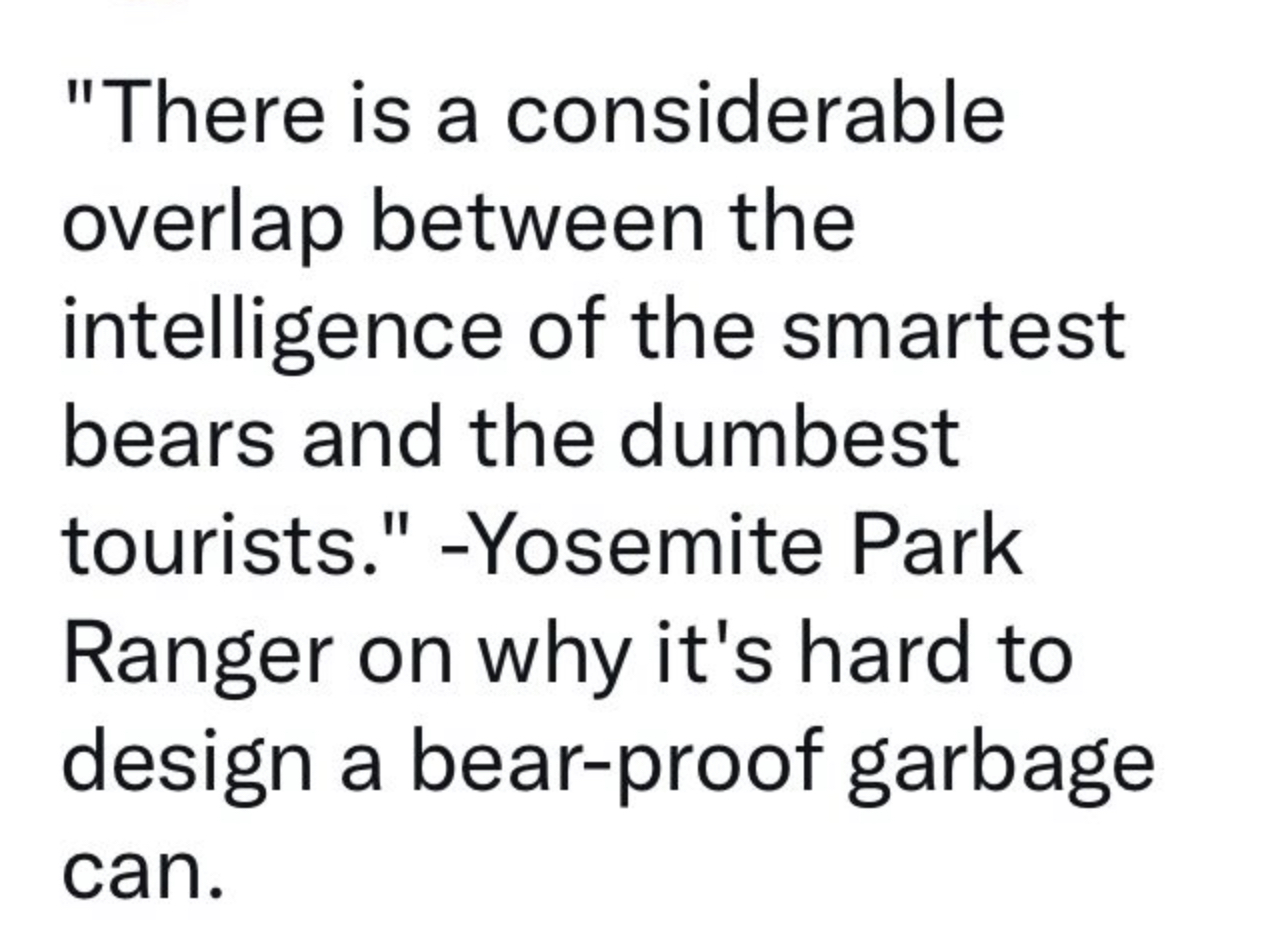
\includegraphics[width=0.382\textwidth]{pictures/schnittmenge.jpeg}
  \end{center}
\caption{Schnittmenge}
\end{wrapfigure}
Die Mengenlehre kann als Fundament der gesamten modernen Mathematik aufgefasst werden. Ihre Begriffe und Sprachelemente sind heute für die Formulierung mathematischer Probleme unentbehrlich geworden.

Die axiomatische Mengenlehre ist ein relativ neuer mathematischer Gegenstand. Die wichtigsten Grundbegriffe gehen auf den deutschen Mathematiker \textsc{Georg Cantor} (1845--1918) zurück. Seine erste mengentheoretische Arbeit erschien 1874. Nach einem Ausspruch von \textsc{David Hilbert}, einem bedeutenden deutschen Mathematiker (1862--1943), schuf \textsc{Cantor} mit seiner Mengenlehre
\begin{quote}
\glqq\dots einen der fruchtreichsten und kräftigsten Wissenszweig der Mathematik, ein Paradies, aus dem uns niemand soll vertreiben kännen.\grqq
\end{quote}

\subsection{Definition der Menge nach Cantor}
Unsere Sprache enthält viele Ausdrücke zur Bezeichnung von Mengen. Die Mathematiker bevorzugen die, etwas unscharfe, 
\begin{cdef}[Menge]
Unter einer Menge versteht man jede Zusammenfassung von bestimmten wohlunterscheidbaren Objekten unserer Anschauung oder unseres Denkens zu einem Ganzen.
\end{cdef}

\begin{bem}
Es ist empfehlenswert, eine \definition{leere Menge} zu definieren. Die leere Menge $\{\}=:\emptyset$ ist die Menge, die kein Element enthält.
\end{bem}

Es gibt zwei Möglichkeiten, eine Menge hinzuschreiben:
\begin{itemize}
\item die \definition{aufzählende} Form
\item die \definition{beschreibende} Form
\end{itemize}

\begin{cdef}[Element]
Die Objekte einer Menge nennt man Elemente der Menge.
\end{cdef}

Es seien $a_1,a_2,a_3,\dots,a_n$ Objekte. Diese lassen sich zu einer Menge $\mathbb{G}$ zusammenfassen.
Elemente einer Menge werden in geschweifte Klammern gefasst. Man schreibt
$$\mathbb{G}=\{a_1,a_2,a_3,\dots,a_n\}$$
\begin{bsp}
Die Menge der fünf traditionellen Sinne
$$\mathbb{S}=\{\text{sehen},\text{hören},\text{riechen},\text{schmecken},\text{tasten}\}$$
\end{bsp}
Mengen bezeichnet man üblicherweise mit Grossbuchstaben, Elemente mit Kleinbuchstaben. Zur Veranschaulichung benutzt man meist sogenannte \definition{Euler}- oder \definition{Venndiagramme}.

\begin{bem}
Um auszudrücken, ob ein Element zu einer Menge $\mathbb{G}$ gehört oder nicht, benutzt man die Symbole $\in$ (sprich \glqq ist Element von\grqq, oder kurz \glqq in\grqq) bzw. $\notin$ (sprich \glqq ist nicht Element von\grqq, oder kurz \glqq nicht in\grqq).
\end{bem}

\begin{figure}
\begin{center}
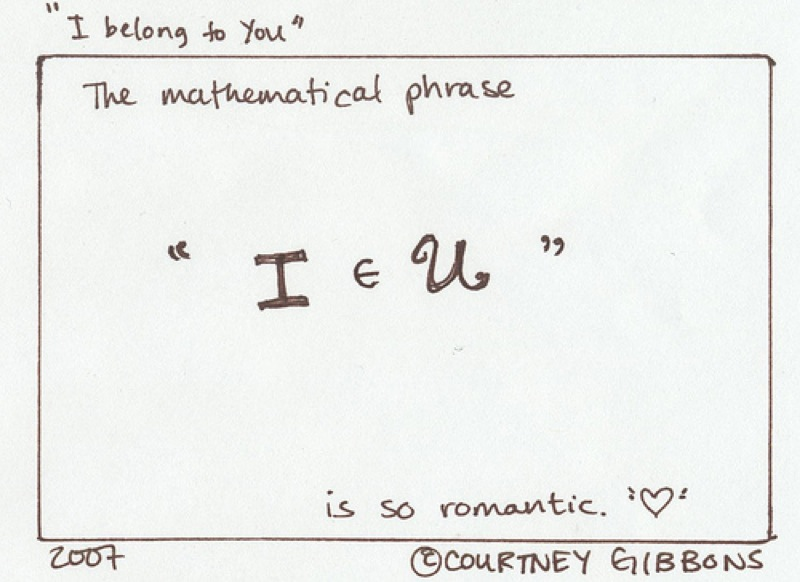
\includegraphics[width=0.45\textwidth]{pictures/belongsto}
\caption{\glqq ist Element von\grqq}
\end{center}
\end{figure}

\begin{uebenv}{inornotin}
Entscheide, ob es sich um eine Menge im mathematischen Sinn handelt. Begründe deine Antwort.
\begin{enumerate}[a)]
\item Alle Primzahlen kleiner als $20$.
\item Alle reichen Leute in der Schweiz.
\item Die Menge der Patienten eines Spitals.
\item Die Bremer Stadtmusikanten aus dem gleichnamigen Märchen.
\end{enumerate}
\end{uebenv}



\begin{uebenv}{explizit}
Schreibe die folgenden Mengen explizit auf. 
\begin{enumerate}[a)]
\item Die Menge der Primzahlen kleiner als $10$
\item Die Menge natürlicher Satelliten der Erde
\end{enumerate}
\end{uebenv}



\begin{uebenv}{inworten}
Gib eine Beschreibung in Worten der folgenden Mengen an und füge jeweils ein weiteres Element hinzu:
\begin{enumerate}[a)]
\item $\{a,e,i,o,\quad\}$
\item $\{1972,1976,1980,\quad\}$
\item $\{2,4,8,16,32,\quad\}$
\end{enumerate}
\end{uebenv}



\begin{uebenv}{mississippi}
Schreibe als Menge:
\begin{enumerate}[a)]
\item die Buchstaben im Wort Mississippi
\item Grossbuchstaben mit einem Symmetriezentrum
\end{enumerate}
\end{uebenv}




\begin{uebenv}{inornotindots}
Es sei $\mathbb{A}$ die Menge der Konsonanten, $\mathbb{B}$ die Menge der Vielfachen von $5$ und
$$\mathbb{C}=\{x\in\mathbb{R}\,|\,(x-5)(x+3)(x-2)=0\}.$$
Setze das richtige Zeichen ($\in$ oder $\notin$).
\begin{enumerate}[a)]
\item $d\quad\mathbb{A}$
\item $5\quad\mathbb{C}$
\item $99\quad\mathbb{B}$
\end{enumerate}
\end{uebenv}



\subsection{Historisches zu Zahlen}

\begin{wrapfigure}{r}{0.4\textwidth}
  \begin{center}
    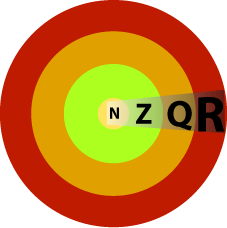
\includegraphics[width=0.3\textwidth]{pictures/zahlen}
  \end{center}
%\caption{A gull}
\end{wrapfigure}
Beim Zählen benutzte der Mensch die Finger, wie dies heute noch Naturvölker oder Kinder tun. Dies spiegelt sich auch in den alten Zahlenzeichen wieder. Häufig waren dies Striche oder Kerben.

Alte Kulturvölker wie die Babylonier, Ägypter oder Römer schufen bestimmte Symbole für die Zahlen $1,5,10,100,1000$ u.a. und bildeten damit durch Aneinanderreihen die übrigen natürlichen Zahlen.

Die Inder gaben diesen Ziffern einen Stellenwert und erfanden für eine leere Stelle ein besonderes Zeichen, die Null. Ein Stellenwertsystem und ein Zeichen für die Null hatten lange vor den Indern auch schon die Babylonier. Bei ihnen war $60$ die Grundzahl (Sexagesimalsystem).

\subsection{Bezeichnungen}

Hier werden folgend übliche Bezeichnungen und Notationen betreffend Zahlenmengen aufgeführt.

Die Menge der \definition{natürlichen Zahlen} wird mit
$$\mathbb{N}=\{1,2,3,\dots\}$$
abgekürzt.

Bei der Subtraktion von $3-3$ oder $4-5$ treten Schwierigkeiten auf, denn die Ergebnisse sind nicht mehr in den natürlichen Zahlen enthalten. Man erhält so die Menge der \definition{ganzen Zahlen}
$$\mathbb{Z}=\{\dots,-3,-2,-1,0,1,2,3,\dots\}.$$

Bei der Behandlung nichttrivialer Divisionen, wie etwa $2\div3$, entsteht ein weiteres Mal das Bedürfnis, das Zahlensystem zu erweitern. Zur Menge der ganzen Zahlen kommen die Brüche hinzu. Damit erhält man die Menge der \definition{rationalen Zahlen}
$$\mathbb{Q}=\{\frac{a}{b}\,|\,a\in\mathbb{Z}, b\in\mathbb{N}\}$$
In dieser Zahlenmenge kännen die vier Grundoperationen $+,-,\cdot,\div$ uneingeschränkt durchgeführt werden; ausser die Division durch $0$. Man sagt:
\begin{quote}
$\mathbb{Q}$ ist \definition{abgeschlossen} bezüglich allen vier Grundoperationen.
\end{quote}

\begin{bem}
Jede rationale Zahl lässt sich durch Division in einen Dezimalbruch verwandeln und vice versa.
\end{bem}

Dabei treten zwei Fälle auf:
\begin{itemize}
\item Nach endlich vielen Schritten tritt der Rest $0$ auf, d.h. der Dezimalbruch ist \definition{abbrechend}.
\item Der Rest $0$ tritt nie auf. Dann heisst der Dezimalbruch \definition{periodisch}.
\end{itemize}
\begin{bsp}
Die rationale Zahl
$$\frac{1}{8}=0.125$$
ist abbrechend. Dagegen ist
$$\frac{1}{7}=0.\overline{142857}$$
periodisch.
\end{bsp}
\begin{uebenv}{schriftlichedivision}
Kannst du obige Beispiele mit schriftlicher Division bestätigen?
\end{uebenv}



\begin{bem}
Umgekehrt lässt sich jeder abbrechende oder periodische Dezimalbruch in einen gewöhnlichen Bruch verwandeln.
\end{bem}

\begin{bsp}
Bei den abbrechenden Dezimalbrüchen ist die Umwandlung einfach. Man bestimmt die Grässe der letzten Nachkommastelle, schreibt als Bruch und kürzt gegebenenfalls:
$$0.25=\frac{25}{100}=\frac{1}{4}$$
Bei den periodischen hilft folgendes Vorgehen: Man definiert die gesuchte Zahl, die als Bruch dargestellt werden soll als $x$. Danach bestimmt man die Länge der Periode und den Wert des Vielfachen von $x$ mit der Periodenlänge. Anschliessend wird $x$ von diesem Produkt abgezogen und die entstandene Gleichung nach $x$ aufgeläst; voilˆ.
\begin{align}
0.\overline{12}&=x \notag\\ \notag
12.\overline{12}&=100x\\ \notag
12&=99x\\ \notag
\frac{12}{99}&=x\\ \notag
\frac{4}{33}&=x
\end{align}
\end{bsp}

\begin{bsp}
Es gibt aber offensichtlich Dezimalbrüche, die weder abbrechend noch periodisch sind.
$$0.1234567891011121314\dots$$
\end{bsp}

\begin{uebenv}{konstruiereirrational}
Kannst du einen nicht periodischen und nicht abbrechenden Dezimalbruch konstruieren, der nur Nullen und Einsen enthält?
\end{uebenv}



Ein weiteres berühmtes Beispiel für eine nicht rationale Zahl ist die positive Zahl, deren Quadrat gleich $2$ ist, nämlich $\sqrt{2}$. Mit der folgenden Argumentation (indirekte Beweismethode)
\marginnote{
<<<<<<< Updated upstream
\qrcode{
https://www.youtube.com/watch?v=_ONbuGauF9I}
=======
\href{https://www.youtube.com/watch?v=_ONbuGauF9I}{\qrcode{https://www.youtube.com/watch?v=_ONbuGauF9I}}
>>>>>>> Stashed changes
}
lässt sich dies leicht einsehen.

\begin{csatz}[Es gibt irrationale Zahlen]{satz:sqrt2irrational}
$\sqrt{2}$ ist nicht rational.
\end{csatz}

\begin{proof}
Wir wollen zeigen, dass $\sqrt{2}$ nicht rational ist. Dazu nehmen wir das Gegenteil der Behauptung an. Kännen wir diese Gegenannahme auf einen Widerspruch führen, so muss die Gegenannahme falsch und somit die ursprüngliche Aussage richtig sein. (Tertium non datur)

Annahme $\sqrt{2}$ ist rational. Also gibt es eine Darstellung
$$\sqrt{2}=\frac{p}{q}$$
wobei $p,q\in\mathbb{N}$ und der Bruch vollständig gekürzt ist. Daraus folgt durch Quadrieren und Multiplizieren mit $q^2$
$$2q^2=p^2$$
Das bedeutet, dass $p^2$, und damit $p$ eine gerade Zahl ist. Andererseits gilt
$$q^2=\frac{p^2}{2}=p\cdot\frac{p}{2}$$
Also ist $q^2$ und damit $q$ gerade. Widerspruch zur Annahme, dass $\frac{p}{q}$ vollständig gekürzt sei. Denn der Bruch kann sicher mit $2$ gekürzt werden, weil sowohl $p$ als auch $q$ gerade sind. Also ist $\sqrt{2}$ nicht rational.
\end{proof}

Diese und andere Tatsachen führen dazu, dass man eine umfassendere Zahlenmenge braucht. Wir geben hier keine formale Definition, sondern beschreiben sie folgendermassen.

\begin{cdef}[Reelle Zahlen]
Die reellen Zahlen entsprechen eindeutig sämtlichen Punkten der Zahlengeraden.
\end{cdef}

Demnach ist also auch jede rationale Zahl eine reelle. Wir unterscheiden noch durch
\begin{cdef}[Irrationale Zahlen]
Reelle Zahlen, die nicht rational sind, heissen irrational.
\end{cdef}

\begin{uebenv}{eulerdiagramm}
Kannst du die Situation aller oben vorgestellten Zahlenmengen $\mathbb{N}$, $\mathbb{Z}$, $\mathbb{Q}$, $\mathbb{R}$ und $\mathbb{I}$ in einem Eulerdiagramm skizzieren?
\end{uebenv}



\begin{uebenv}{schriftlichdividieren}
Berechne mit Hilfe der schriftlichen Division den Wert von
\begin{enumerate}[a)]
    \item $\frac{1}{16}$
    \item $\frac{1}{15}$
    \item $\frac{3}{11}$
    \item $\frac{1}{7}$
\end{enumerate}

\end{uebenv}




\begin{uebenv}{runterbrechen}
Schreibe als rationale Zahl in Bruchform
\begin{enumerate}[a)]
    \item $0.1234$
    \item $0.\overline{3}$
    \item $0.\overline{14}$
    \item $0.1\overline{23}$
    \item $2.\overline{9}$
\end{enumerate}
\end{uebenv}




\begin{uebenv}{zahlengerade}
Konstruiere auf einer Zahlengerade die Punkte
\begin{enumerate}[a)]
    \item $\sqrt{5}$
    \item $\frac{2}{3}$
    \item $-1\frac{1}{4}$
    \item $-\sqrt{3}$
    \item $0.\overline{7}$
\end{enumerate}

\end{uebenv}




\subsection{Kardinalität einer Menge}
\begin{figure}
  \begin{center}
    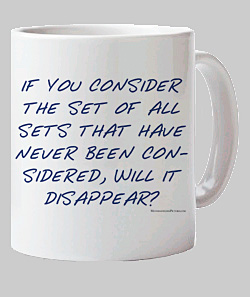
\includegraphics[width=0.382\textwidth]{pictures/sets}
  \end{center}
\caption{Is there a set of non considered sets?}
\end{figure}
Im täglichen Leben verwendet man die natürlichen Zahlen vor allem
\begin{itemize}
\item zum Nummerieren/Ordnen von Gegenständen; die natürlichen Zahlen dienen als \definition{Ordinalzahlen}.
\item als Anzahlen zur grössenmässigen Beschreibung von Mengen; als \definition{Kardinalzahlen}.
\end{itemize}

Wenn man Elemente einer Menge $\mathbb{G}$ abzählt, so ist die letzte Zahl zugleich die Anzahl der Elemente dieser Menge.

\begin{cdef}[Kardinalität]
Die Anzahl der Elemente einer Menge $\mathbb{G}$ heisst \emph{Kardinalität} oder Mächtigkeit von $\mathbb{G}$. Man schreibt $\text{card}(\mathbb{G})$.
\end{cdef}

\begin{bsp}
Für $\mathbb{G}=\{-2,-1,0,1,2\}$ ist $\text{card}(\mathbb{G})=5$. Oder man hat $\text{card}(\mathbb{\emptyset})=0$.
\end{bsp}

\subsection{Teilmenge}

\begin{cdef}[Teilmenge]
Ist
\marginnote{
<<<<<<< Updated upstream
\qrcode{
https://www.youtube.com/watch?v=FDNt0pE4jUA}
=======
\href{https://www.youtube.com/watch?v=FDNt0pE4jUA}{\qrcode{https://www.youtube.com/watch?v=FDNt0pE4jUA}}
>>>>>>> Stashed changes
}
jedes Element einer Menge $\mathbb{A}$ auch in einer Menge $\mathbb{B}$ enthalten, so ist $\mathbb{A}$ eine \emph{Teilmenge} von $\mathbb{B}$. Man schreibt
$$\mathbb{A}\subset\mathbb{B}\text{ oder auch }\mathbb{A}\subseteq\mathbb{B}$$
\end{cdef}


\begin{csatz}[Leere Menge]
Die
\marginnote{
<<<<<<< Updated upstream
\qrcode{
https://www.youtube.com/watch?v=SYxQy0rDctg}
=======
\href{https://www.youtube.com/watch?v=SYxQy0rDctg}{\qrcode{https://www.youtube.com/watch?v=SYxQy0rDctg}}
>>>>>>> Stashed changes
}
leere Menge ist Teilmenge jeder Menge.
\end{csatz}

\begin{proof}
Gegenannahme: Wäre die leere Menge nicht Teilmenge jeder Menge, dann gäbe es mindestens eine Menge, sagen wir $\mathbb{M}$, welche die leere Menge nicht enthalten würde. Dann müsste es aber nach Definition von Teilmenge ein Element $x$ in der leeren Menge geben, das nicht zu $\mathbb{M}$ gehärt. Widerspruch, denn somit wäre die leere Menge ja nicht leer, weil sie dieses $x$ enthalten würde. Also muss die leere Menge Teilmenge jeder Menge sein.
\end{proof}

Haben zwei Mengen $\mathbb{A}$ und $\mathbb{B}$ die gleichen Elemente, so schreibt man $\mathbb{A}=\mathbb{B}$.

\subsection{Operationen}
\marginnote{
<<<<<<< Updated upstream
\qrcode{
https://www.youtube.com/watch?v=nvYwG5cJGWA}
=======
\href{https://www.youtube.com/watch?v=nvYwG5cJGWA}{\qrcode{https://www.youtube.com/watch?v=nvYwG5cJGWA}}
>>>>>>> Stashed changes
}
\subsubsection{Durchschnittsmenge}
\begin{cdef}[Schnitt]
Die Durchschnittsmenge zweier Mengen $\mathbb{A}$ und $\mathbb{B}$ besteht aus sämtlichen Elementen, die sowohl zu $\mathbb{A}$ als auch zu $\mathbb{B}$ gehären. In mathematischer Schreibweise
$$\mathbb{A}\cap\mathbb{B}=\{x\mid x\in\mathbb{A}\text{ und }x\in\mathbb{B}\}$$
\end{cdef}

\def\firstcircle{(0,0) circle (1.5cm)}
\def\secondcircle{(0:2cm) circle (1.5cm)}
\def\grundmenge{(-3,-2) rectangle (3,2)}

\colorlet{circle edge}{darkblue!50}
\colorlet{circle area}{darkblue!20}

\colorlet{rectangle edge}{darkblue!50}
\colorlet{rectangle area}{darkblue!20}

\tikzset{filled/.style={fill=circle area, draw=circle edge, thick},
    outline/.style={draw=circle edge, thick}}

% Set A and B
\begin{center}
\begin{tikzpicture}
    \begin{scope}
        \clip \firstcircle;
        \fill[filled] \secondcircle;
    \end{scope}
    \draw[outline] \firstcircle node {$\mathbb{A}$};
    \draw[outline] \secondcircle node {$\mathbb{B}$};
    \node[anchor=south] at (current bounding box.north) {$\mathbb{A} \cap \mathbb{B}$};
\end{tikzpicture}
\end{center}

\begin{bsp}
Ist $\mathbb{A}=\{1,2\}$ und $\mathbb{B}=\{2,3\}$, dann gilt
$$\mathbb{A}\cap\mathbb{B}=\{2\}$$
\end{bsp}
\begin{cdef}[disjunkt]
Zwei Mengen heissen \emph{disjunkt}, wenn sie keine gemeinsamen Elemente haben, d.~h.
$$\mathbb{A}\cap\mathbb{B}=\emptyset$$
\end{cdef}

\pagebreak

\subsubsection{Vereinigungsmenge}
\begin{cdef}[Vereinigung]
Die \emph{Vereinigunsmenge} zweier Mengen $\mathbb{A}$ und $\mathbb{B}$ besteht aus sämtlichen Elementen, die zu $\mathbb{A}$ oder $\mathbb{B}$ gehären. Man schreibt
$$\mathbb{A}\cup\mathbb{B}=\{x\mid x\in\mathbb{A}\text{ oder }x\in\mathbb{B}\}$$
\end{cdef}

\begin{center}
% Set A or B
\begin{tikzpicture}
    \draw[filled] \firstcircle node {$\mathbb{A}$}
                  \secondcircle node {$\mathbb{B}$};
    \node[anchor=south] at (current bounding box.north) {$\mathbb{A} \cup \mathbb{B}$};
\end{tikzpicture}
\end{center}

\begin{bsp}
Für $\mathbb{A}$ und $\mathbb{B}$ wie im obigen Beispiel gilt
$$\mathbb{A}\cup\mathbb{B}=\{1,2,3\}$$
\end{bsp}

\subsubsection{Differenzmenge}
\begin{cdef}[Differenz]
Die Differenzmenge von $\mathbb{A}$ mit $\mathbb{B}$ besteht aus sämtlichen Elementen, die zu $\mathbb{A}$, aber nicht zu $\mathbb{B}$ gehären. Man schreibt
$$\mathbb{A}\setminus\mathbb{B}=\{x\mid x\in\mathbb{A}\text{ und }x\notin\mathbb{B}\}$$
\end{cdef}

\begin{center}
% Set A but not B
\begin{tikzpicture}
    \begin{scope}
        \clip \firstcircle;
        \draw[filled, even odd rule] \firstcircle node {$\mathbb{A}$}
                                     \secondcircle;
    \end{scope}
    \draw[outline] \firstcircle
                   \secondcircle node {$\mathbb{B}$};
    \node[anchor=south] at (current bounding box.north) {$\mathbb{A}\setminus \mathbb{B}$};
\end{tikzpicture}
\end{center}

\begin{bsp}
Mit $\mathbb{A}$ und $\mathbb{B}$ wie oben gilt
$$\mathbb{A}\setminus\mathbb{B}=\{1\}$$
\end{bsp}

\subsubsection{Komplementärmenge}
\begin{cdef}[Komplement]
Es sei $\mathbb{A}\subset\mathbb{G}$. Das \emph{Komplement} von $\mathbb{A}$ bezüglich der Grundmenge $\mathbb{G}$ besteht aus sämtlichen Elementen von $\mathbb{G}$, die nicht zu $\mathbb{A}$ gehären. Man schreibt
$$\overline{\mathbb{A}}=\{x\mid x\in\mathbb{G}\text{ und }x\notin\mathbb{A}\}$$
\end{cdef}

\begin{center}
\begin{tikzpicture}
    \begin{scope}
        \clip \grundmenge;
        \draw[filled, even odd rule] \grundmenge node[anchor=north east] {$\overline{\mathbb{A}}$}
                                     \firstcircle;
    \end{scope}
    \draw[outline] \firstcircle node {$\mathbb{A}$};
    \node[anchor=south] at (current bounding box.north) {$\mathbb{G}$};
\end{tikzpicture}
\end{center}

\begin{bsp}
Ist $\mathbb{G}=\{1,2,3\}$ und $\mathbb{A}$ wie oben, dann gilt
$$\overline{\mathbb{A}}=\{3\}$$
\end{bsp}

\begin{uebenv}{kapitel}
Es seien

\begin{align*}
\mathbb{A}&=\{k,a,p,i,t,e,l\}\notag\\
\mathbb{B}&=\{t,e,i,l\}\notag\\
\mathbb{C}&=\{k,a,p\}\notag\\
\mathbb{D}&=\{\}\notag\\
\mathbb{E}&=\{e,i,s\}\notag
\end{align*}
Welche der folgenden Aussagen sind richtig?
\begin{enumerate}[a)]
    \item $\mathbb{E}\subset\mathbb{A}$
     \item $\mathbb{A}\subset\mathbb{B}$ \item $\mathbb{B}\subset\mathbb{A}$ \item $\mathbb{D}\subset\mathbb{C}$ \item $\mathbb{C}\subset\mathbb{A}$ \item $\mathbb{E}\subset\mathbb{D}$
\end{enumerate}

\end{uebenv}




\begin{uebenv}{richtigoderfalsch}
Welche der folgenden Aussagen sind richtig?

\begin{enumerate}[a)]
\item $0\notin\emptyset$
\item $0\subset\{0,1,2\}$
\item $\emptyset\in\{1,2,3\}$
\item $\emptyset\subset{0}$
\item $\emptyset=\{x\mid x\neq x\}$
\item $\{1,2\}\not\subset\{2,1\}$
\item $\emptyset\in\{0\}$
\item $\{a\}\in\{a,\{a\}\}$
\item $\emptyset\subset\{\emptyset,\{a\}\}$
\item $\emptyset\in\{\emptyset,\{a\}\}$
\end{enumerate}
\end{uebenv}




\begin{cdef}[Potenzmenge]
Die Menge aller Teilmengen einer Menge $\mathbb{A}$ heisst Potenzmenge von $\mathbb{A}$.
$$\mathcal{P}(\mathbb{A})=\{\mathbb{B}\mid \mathbb{B}\subset\mathbb{A}\}.$$
\end{cdef}

\begin{bsp}
Die Potenzmenge von $\mathbb{A}=\{1,2\}$ ist
$$\mathcal{P}(\mathbb{A})=\{\{\},\{1\},\{2\},\{1,2\}\}$$
\end{bsp}

\begin{uebenv}{potenzmenge}
Bestimme die Potenzmenge $\mathcal{P}(\mathbb{A})$ von
$$\mathbb{A}=\{a,b,c\}$$
\end{uebenv}




\begin{uebenv}{kardinalittpotenzmenge}
Wie viele Elemente hat die Potenzmenge einer Menge $\mathbb{A}$ mit $\text{card}(\mathbb{A})=n$?
\end{uebenv}




\begin{uebenv}{zahlen}
Es sei die Grundmenge
$$\mathbb{G}=\{1,2,3,4,\dots,19,20\}$$
sowie Teilmengen von $\mathbb{G}$

\begin{align*}
\mathbb{A}&=\{x\in\mathbb{G}\mid x\text{ ist Viererzahl}\}\\
\mathbb{B}&=\{8,9,10,11,12,13\}\\
\mathbb{C}&=\{x\in\mathbb{G}\mid x\text{ ist ungerade}\}
\end{align*}

Ermittle

\begin{enumerate}[a)]
    \item $\mathbb{A}\cap\mathbb{B}$
    \item $\mathbb{A}\cap\mathbb{C}$
    \item $\overline{\mathbb{C}\cup\mathbb{B}}$
    \item $\overline{\mathbb{C}}\setminus\mathbb{A}$
\end{enumerate}

\end{uebenv}




\begin{uebenv}{zahlenmengen}
Ermittle

\begin{enumerate}[a)]
    \item $\mathbb{R}\cap\mathbb{Q}$
    \item $(\mathbb{N}\cap\mathbb{Z})\cup\mathbb{Q}$
    \item $\mathbb{R}\cup(\mathbb{Z}\cap\mathbb{Q})$
\end{enumerate}

\end{uebenv}




\begin{uebenv}{ausschluss}
Von $45$ Schülerinnen nehmen $26$ an einer Arbeitsgemeinschaft für Physik, $14$ an einer Arbeitsgemeinschaft für Chemie teil. Wie viele Schülerinnen nehmen mindestens an keiner der beiden Arbeitsgemeinschaften teil, wie viele höchstens?
\end{uebenv}




\begin{uebenv}{etwaslogik}
Betrachte folgende Mengen: Grundmenge
$$\mathbb{G}=\{x\mid x\text{ ist Klubmitglied}\}$$

\begin{align*}
\mathbb{A}&=\{x\mid x\text{ trägt eine Krawatte}\}\\
\mathbb{B}&=\{x\mid x\text{ hat seinen Arbeitsplatz in Basel}\}\\
\mathbb{C}&=\{x\mid x\text{ hat braune Augen}\}\\
\mathbb{D}&=\{x\mid x\text{ ist älter als 20 Jahre}\}
\end{align*}

Übersetze die folgenden beiden Sätze in die Mengensprache:

\begin{enumerate}[a)]
\item Es gibt keine Klubmitglieder mit braunen Augen, die älter als 20 Jahre sind.
\item Alle Klubmitglieder, die eine Krawatte tragen, arbeiten in Basel.
\end{enumerate}
\end{uebenv}



\clearpage

\subsection{Notizen zu den Übungen}

\begin{lsg}{inornotin}
\begin{enumerate}[a)]
    \item \ding{55}, klar definiert $\{2,3,5,7,11,13,17,19\}$
    \item \ding{51}, reich ist als Kriterium nicht stringent genug.
    \item \ding{55}, klar definierte Individuen; man kann entscheiden, ob das Element dazu gehört oder nicht.
    \item Darüber lässt sich streiten. \ding{55}, denn jeder kennt die Bremer Stadtmusikanten. \ding{51}, vielleicht gibt es mehr als einen Esel, der singen kann. Vielleicht kann ich nicht entscheiden, ob dieser oder jener Hahn dazu gehört.
\end{enumerate}
\end{lsg}
\begin{lsg}{explizit}
\begin{enumerate}[a)]
    \item $\{2,3,5,7\}$
    \item $\{\text{Mond}\}$
\end{enumerate}
\end{lsg}
\begin{lsg}{inworten}
    \begin{enumerate}[a)]
        \item Menge der Vokale, $u$.
        \item Menge an Jahrzahlen, an denen Olympische Spiele stattfanden, 1984
        \item Menge der Zweierpotenzen mit natürlichen Exponenten, $64$.
    \end{enumerate}
\end{lsg}
\begin{lsg}{mississippi}
\begin{enumerate}[a)]
    \item $\{M,i,s,p\}$
    \item $\{\texttt{H,I,N,O,S,X,Z}\}$
\end{enumerate}
\end{lsg}
\begin{lsg}{inornotindots}
\begin{enumerate}[a)]
\item $d\in\mathbb{A}$
\item $5\in\mathbb{C}$, da $0\cdot8\cdot3=0$
\item $99\not\in\mathbb{B}$
\end{enumerate}
\end{lsg}
\begin{lsg}{schriftlichedivision}
    Zuerst $1\div8=0$ Rest 1. Dann $10\div8$ ist $1$ Rest $2$. Wieder einen Zehner für eine weitere Stelle opfern: $20\div8=2$ Rest $4$ und $40\div8=5$; insgesamt also $0.125$.

    Bei einem Siebtel rechnet man analog zu oben und kommt so zum Ergebnis aus dem Skript.
\end{lsg}
\begin{lsg}{konstruiereirrational}
    $0.101001000100001\dots$
\end{lsg}
\begin{lsg}{eulerdiagramm}
    Es muss $\mathbb{N}\subset\mathbb{Z}\subset\mathbb{Q}\subset\mathbb{R}$.
\end{lsg}
\begin{lsg}{schriftlichdividieren}
Man kann das Ergebnis mit einem Rechner prüfen. Exemplarisch rechne ich hier
\begin{align*}
    1\div16 &=0.0625\tag{Rest 1,10}\\
    100\div16 &= 6\tag{Rest 4}\\
    40\div16 &= 2\tag{Rest 8}\\
    80\div16 &= 5\tag{Rest 0}
\end{align*}
\end{lsg}
\begin{lsg}{runterbrechen}
Auch hier kann man das Ergebnis wieder mit einem Rechner kontrollieren. Exemplarisch rechne ich hier
\begin{align*}
    x &= 0.1\overline{23}\\
    100x &= 12.3\overline{23}\\
    100x-x &= 12.3\overline{23}-0.1\overline{23}\\
    99x &= 12.2\\
    x &= \frac{12.2}{99} = \frac{122}{990} = \frac{61}{450}
\end{align*}
\end{lsg}
\begin{lsg}{zahlengerade}
\begin{enumerate}[a)]
    \item Verwende Pythagoras $\sqrt{5}=\sqrt{1^2+2^2}$
    \item Mit Strahlensatz: Man ziehe von $0$ aus einen Strahl und trage $3$ gleichlange Strecken ab. Den Endpunkt verbindet man nun mit $1$. Die Parallelen zu dieser Strecke, welche durch die Markierungen gehen, teilen das Intervall $[0,1]$ in Drittel.
    \item Man trägt rückwärts ab und konstruiert einen Viertel analog zu einem Drittel.
    \item $\sqrt{3}=\sqrt{1^2+(\sqrt{2})^2}$ und $\sqrt{2}=\sqrt{1^2+1^2}$ konstruieren wir auch mit dem Pythagoras.
    \item Wir können berechnen, dass $0.\overline{7}=\frac{7}{9}$ ist und konstruieren Neuntel so wie oben die Drittel.
\end{enumerate}
\end{lsg}
\begin{lsg}{kapitel}
\begin{enumerate}[a)]
    \item \ding{55}, $s\not\in\mathbb{A}$
    \item \ding{55}, $k,a,p\not\in\mathbb{B}$
    \item \ding{51}
    \item \ding{51}
    \item \ding{51}
    \item \ding{55}, $e,i,s\not\in\mathbb{D}$
\end{enumerate}
\end{lsg}
\begin{lsg}{richtigoderfalsch}
\begin{enumerate}[a)]
\item \ding{51}
\item \ding{55}, $0$ ist keine Menge.
\item \ding{55}, das Element $\emptyset$ kommt nicht vor.
\item \ding{55}, $0$ ist keine Menge.
\item \ding{51}
\item \ding{55}, das Element $\emptyset$ kommt nicht vor.
\item \ding{55}, $\{1,2\}=\{2,1\}$
\item \ding{51}
\item \ding{51}
\item \ding{51}
\end{enumerate}
\end{lsg}
\begin{lsg}{potenzmenge}
$\mathcal{P}(\mathbb{A})=\{\{\},\{a\},\{b\},\{c\},\{a,b\},\{a,c\},\{b,c\},\mathbb{A}\}$
\end{lsg}
\begin{lsg}{kardinalittpotenzmenge}
Sei $K$ die Anzahl Elemente der Potenzmenge. Wir wissen die ersten paar Zuordnungen $(n\mid K)$:
$$(0\mid 1),(1\mid 2),(2\mid 4),(3\mid 8)$$
Fügt man zur Menge $\mathbb{A}$ ein weiteres Element hinzu, so nimmt die Anzahl möglicher Mengenkombinationen um den Faktor $2$ zu. Denn jede bereits vorhandene Menge, kann mit dem neuen Element kombiniert werden, woraus sich $2n$ Elemente für die neue Potenzmenge ergeben. Wir haben also $K=2n$ Elemente in der Potenzmenge für eine Menge mit $n$ Elementen.
\end{lsg}
\begin{lsg}{zahlen}
\begin{enumerate}[a)]
    \item $\mathbb{A}\cap\mathbb{B}=\{8,12\}$
    \item $\mathbb{A}\cap\mathbb{C}=\{\}$
    \item $\overline{\mathbb{C}\cup\mathbb{B}}=\{2,4,6,14,16,18,20\}$, da $\mathbb{C}\cup\mathbb{B}=\{1,3,5,7,8,9,10,11,12,13,15,17,19\}$
    \item $\overline{\mathbb{C}}\setminus\mathbb{A}=\{2,6,10,14,18\}$
\end{enumerate}
\end{lsg}
\begin{lsg}{zahlenmengen}
\begin{enumerate}[a)]
    \item $\mathbb{R}\cap\mathbb{Q}=\mathbb{Q}$
    \item $(\mathbb{N}\cap\mathbb{Z})\cup\mathbb{Q}=\mathbb{N}\cup\mathbb{Q}=\mathbb{Q}$
    \item $\mathbb{R}\cup(\mathbb{Z}\cap\mathbb{Q})=\mathbb{R}\cup\mathbb{Z}=\mathbb{R}$
\end{enumerate}
\end{lsg}
\begin{lsg}{ausschluss}
Will ich möglichst viele Schülerinnen, die an keiner der beiden Arbeitsgemeinschaften teilnehmen, dann kommen alle $14$ der Chemie in den Schnitt mit der Physik. Dies ergibt dann $45-26=19$ Leute.

Für möglichst wenige Schülerinnen in Arbeitsgemeinschaften lassen wir den Schnitt von Chemie und Physik leer: $45-(24+16)=5$.
\end{lsg}
\begin{lsg}{etwaslogik}
\begin{enumerate}[a)]
    \item $\mathbb{C}\cap\mathbb{D}=\emptyset$
    \item $\mathbb{A}\subseteq\mathbb{B}$
\end{enumerate}
\end{lsg}

\clearpage

\section{Polynome und Brüche}

\subsection{Grundlagen}

Polynome und Bruchterme bilden die Bausteine vieler Berechnungen und mathematischer Theorien. Deshalb gehört die Fähigkeit --- mit Polynomen und Brüchen sicher umgehen zu können --- zu den grundlegendsten Voraussetzungen, um Technik und Anwendungen der Neuzeit verstehen zu können. Als Einstieg zu den Polynomen betrachten wir erst \definition{das Pascal'sche Dreieck}.

\begin{wrapfigure}{r}{0.4\textwidth}
  \begin{center}
    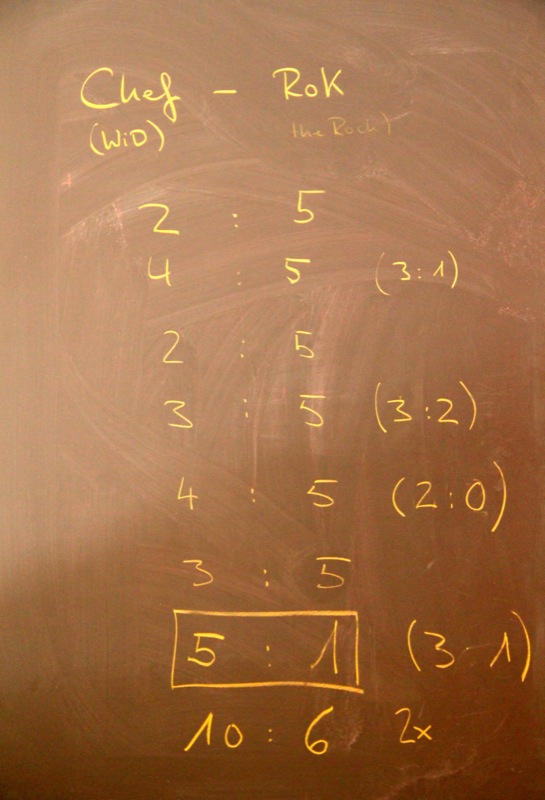
\includegraphics[width=0.22\textwidth]{pictures/rokwidboard}
  \end{center}
%\caption{A gull}
\end{wrapfigure}

\subsection{Das Pascal'sche Dreieck}

\begin{uebenv}{binompotenzen}
Multipliziere aus.
    \begin{enumerate}[a)]
      \item $(a+b)^0$
      \item $(a+b)^1$
      \item $(a+b)^2$
      \item $(x-y)^3$
      \item $(-u+2v)^4$
    \end{enumerate}
  \end{uebenv}
  
Im Folgenden sollen nun das Pascal-Dreieck und einige seiner Eigenschaften präsentiert werden.

Das Pascal'sche Dreieck sieht wie folgt aus; es kann theoretisch unendlich \glqq hoch\grqq\ werden.

  \begin{center}
    \ \\[2pt]
    $1$\\[6pt]
    $1\quad\quad1$\\[6pt]
    $1\quad\quad2\quad\quad1$\\[6pt]
    $1\quad\quad3\quad\quad3\quad\quad1$\\[6pt]
    $1\quad\quad4\quad\quad6\quad\quad4\quad\quad1$\\[6pt]
    $1\quad\quad5\quad\quad10\quad\quad10\quad\quad5\quad\quad1$\\[6pt]
    $1\quad\quad6\quad\quad15\quad\quad20\quad\quad15\quad\quad6\quad\quad1$\\[6pt]
    $1\quad\quad7\quad\quad21\quad\quad35\quad\quad35\quad\quad21\quad\quad7\quad\quad1$\\[6pt]
    $\dots$
  \end{center}

Offensichtlich besteht das Dreieck aus lauter $1$-en am Rand. In jeder folgenden Zeile nimmt die Anzahl der Zahlen um Eins zu. Die Zahl in der unteren Zeile ist gleich der Summe der darüber liegenden Zahlen.

Ferner sehen wir, dass diese Zahlen stets der Koeffizienten der Summanden des ausmultiplizierten Terms $(a+b)^n$ sind.


  \begin{align}
    (a+b)^0 &= 1\notag\\
    (a+b)^1 &= a+b\notag\\
    (a+b)^2 &= a^2+2ab+b^2\notag\\
    (a+b)^3 &= a^3+3a^2b+3ab^2+b^3\notag\\
    (a+b)^4 &= a^4+4a^3b+6a^2b^2+4ab^3+b^4\notag\\
    \dots &\dots\notag
  \end{align}

\begin{uebenv}{binomialkoeffizient}
    Theoretisch kann man die $k$-te Zahl in der $n$-ten Zeile auch direkt berechnen. Finde eine Formel.
\end{uebenv}

Das Pascal-Dreieck besitzt unter anderem folgende Eigenschaften
\begin{itemize}
\item In der Diagonalen $1,3,6,10,15,\dots$ liest man die Dreieckszahlen ab.
\item Die Summe der $n$-ten Zeile entspricht der Zweierpotenz $2^{n}$.
\item Das Verhältnis zweier benachbarter Zahlen einer Zeile entspricht dem Verhältnis der Anzahl Zahlen, die links und rechts davon stehen inklusive.
\end{itemize}

\begin{uebenv}{direktpascal}
Berechne mit Hilfe des Pascal'schen Dreieck

\begin{enumerate}[a)]
\item $(x-1)^5$
\item $(-3+2c)^3$
\item $(y^3-2)^3$
\item $(-x-z)^4$
\end{enumerate}
\end{uebenv}

\subsection{Notizen zu den Übungen}

\begin{lsg}{binompotenzen}
Man notiert die ersten paar Zeilen des Pascal'schen Dreiecks und rechnet:
\begin{enumerate}[a)]
    \item $1$
    \item $a+b$
    \item $a^2+2ab+b^2$
    \item $x^3-3x^2y+3xy^2-y^3$
    \item $1\cdot(-u)^4+4(-u)^3\cdot2v+6(-u)^2\cdot(2v)^2+4(-u)\cdot(2v)^3+1\cdot(2v)^4=u^4-8u^3v+24u^2v^2-32uv^3+16v^4$
\end{enumerate}
\end{lsg}
\begin{lsg}{binomialkoeffizient}
    Wir denken ans Ausmultiplizieren eines Terms $(a+b)^n$ und welcher Summand wie viele Beiträge bekommt. Seien $0\leq k,l\leq n$ natürliche Zahlen. Dann kommt der Summand $a^kb^l$ genau $\frac{n(n-1)(n-2)\dots(n-k+1)}{k!}=\frac{n(n-1)(n-2)\dots(n-l+1)}{l!}$ vor, da ich ja aus $n$ Faktoren $k$ bzw. $l$ kombinieren kann. Man schreibt
    $$\frac{n(n-1)(n-2)\dots(n-k+1)}{k!}=\frac{\frac{n!}{(n-k)!}}{k!}=\frac{n!}{k!(n-k)!}=:\binom{n}{k}$$
    und nennt letzteres einen \definition{Binomialkoeffizienten} (sprich: \glqq n tief k\grqq).
\end{lsg}
\begin{lsg}{direktpascal}
\begin{enumerate}[a)]
    \item $x^5-5x^4+10x^3-10x^2+5x-1$
    \item $(-3)^3+3\cdot(-3)^2(2c)+3(-3)(2c)^2+8c^3=8c^3-36c^2+54c-27$
    \item $y^3-6y^6+12y^3-8$
    \item $x^4+4x^3z+6x^2z^2+4xz^3+z^4$
\end{enumerate}
\end{lsg}

\clearpage

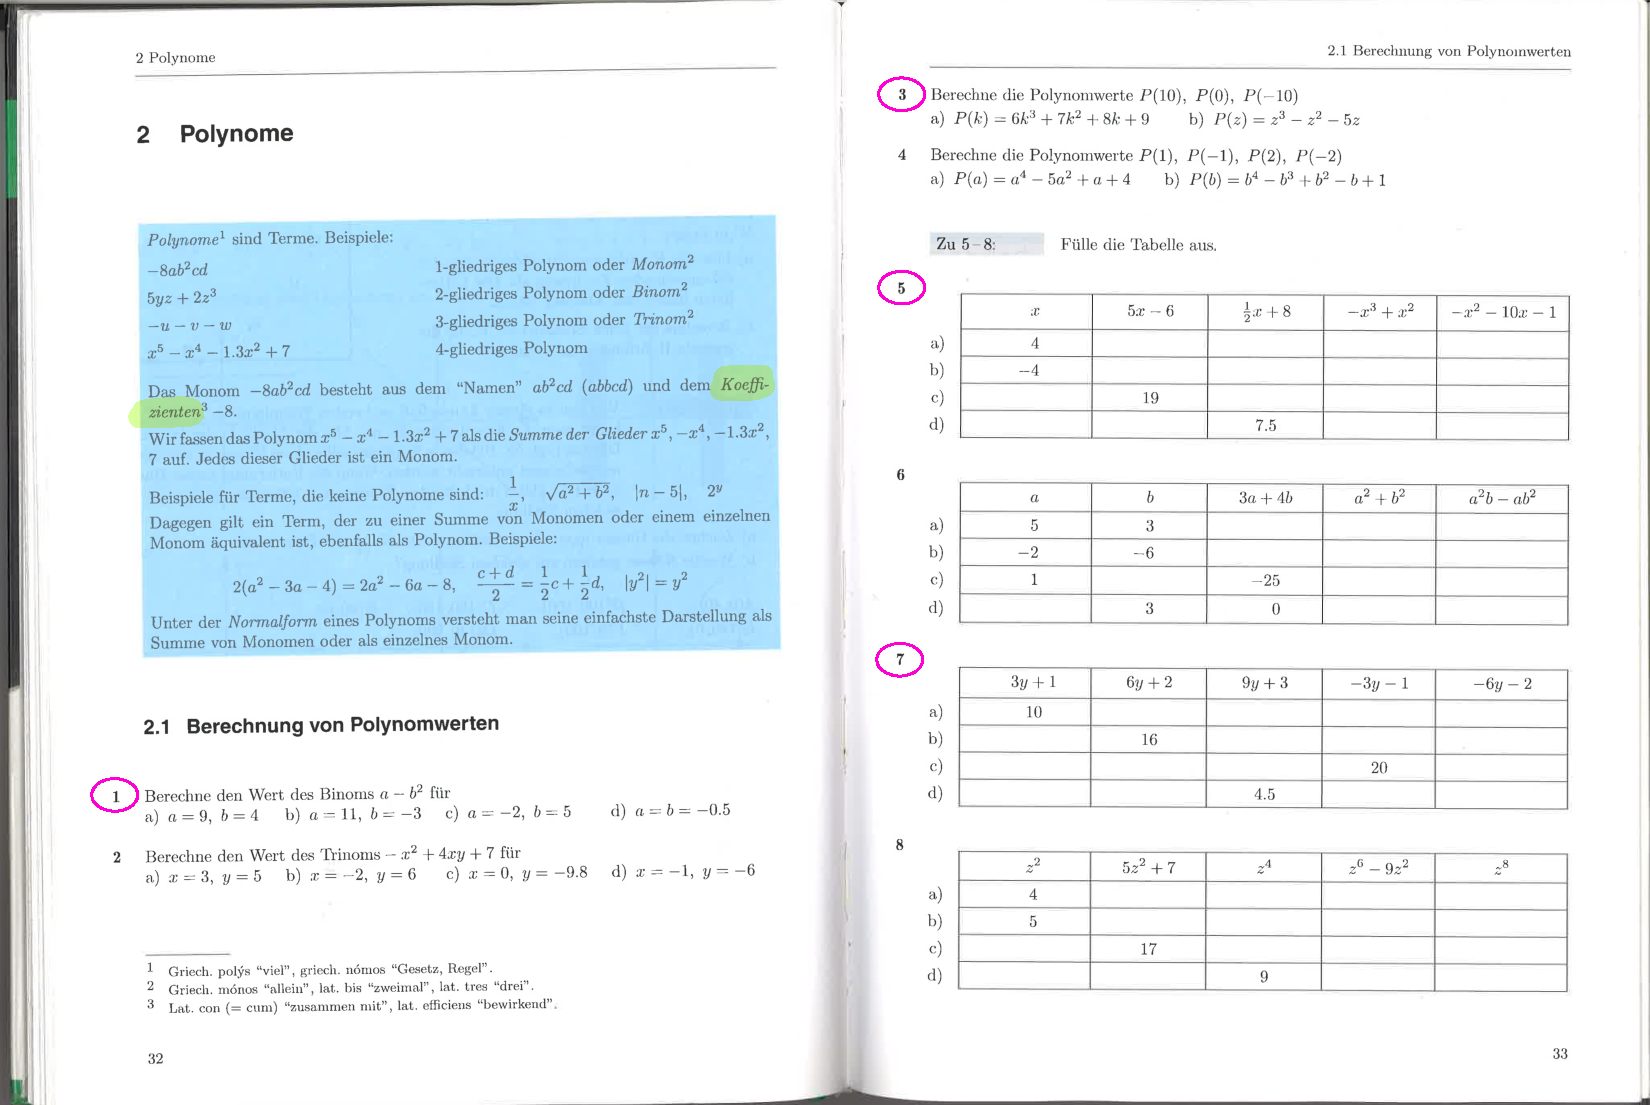
\includepdf[pages=1-2,pagecommand=\subsection{Aufgaben zu Polynome},scale=0.7,nup=1x2]{pictures/Algebra 1 Kapitel 2 Polynome Aufgaben.pdf}
\includepdf[pages=3-12,width=0.8\textheight,nup=1x2]{pictures/Algebra 1 Kapitel 2 Polynome Aufgaben.pdf}

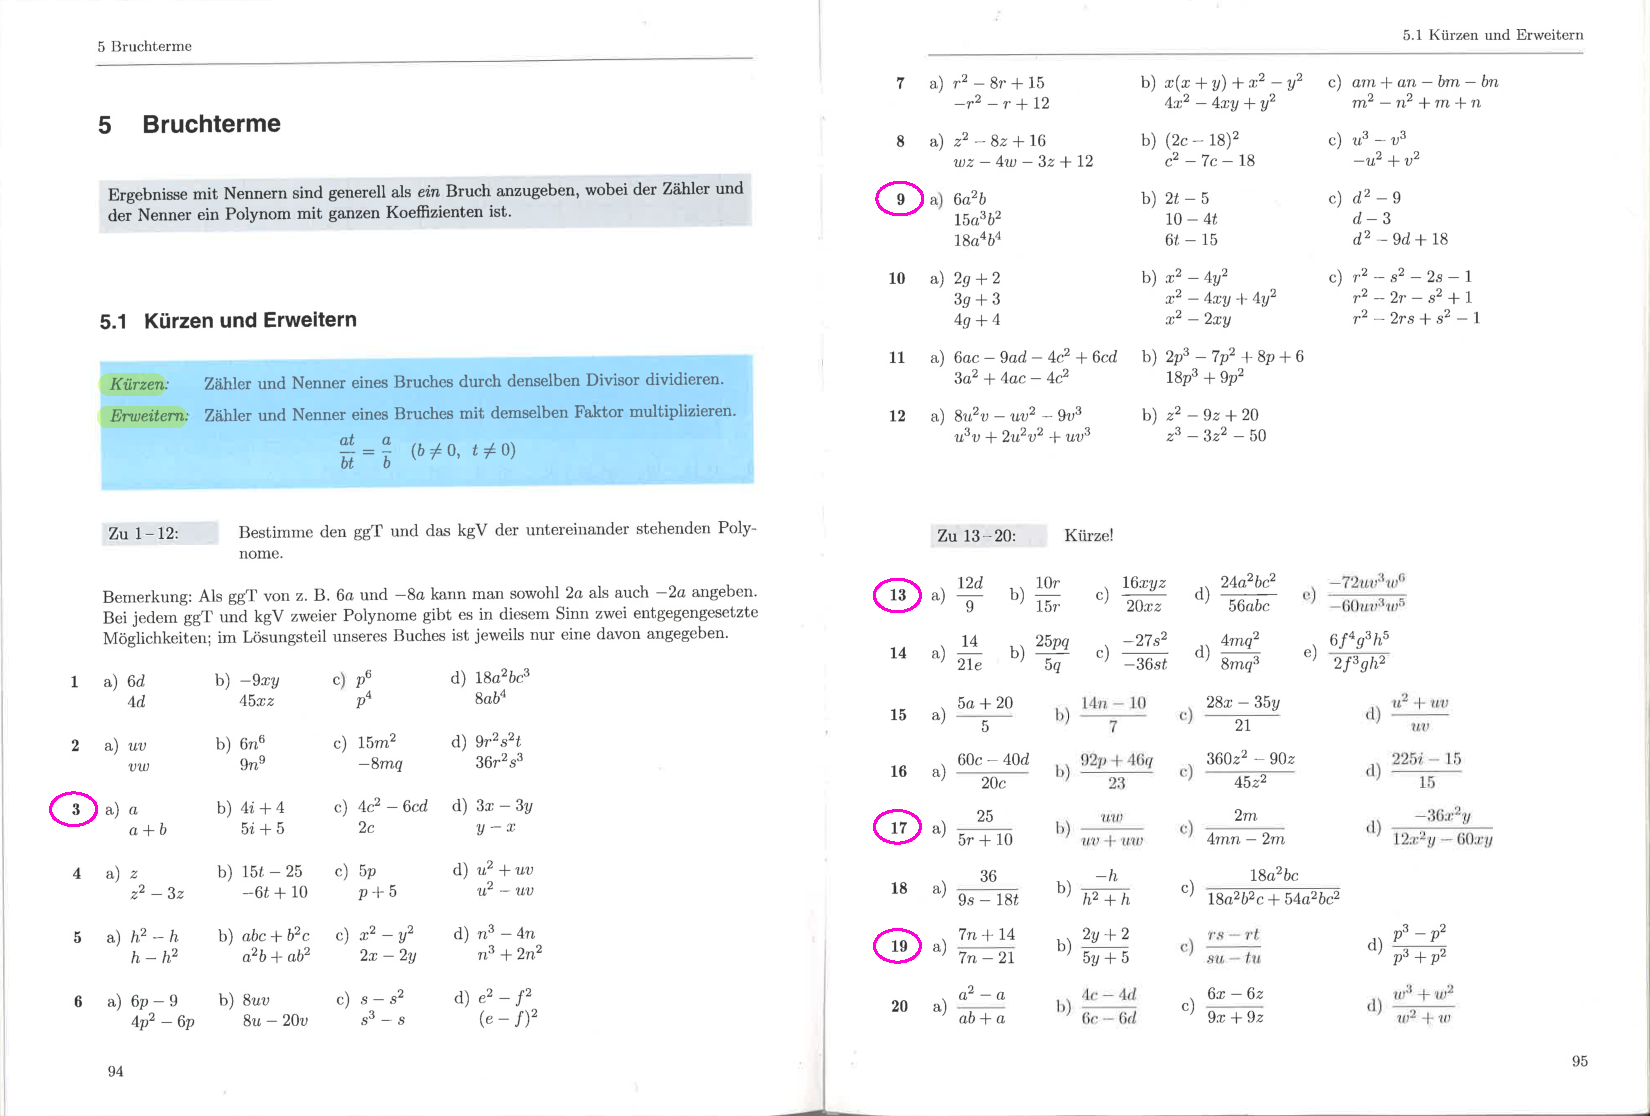
\includepdf[pages=1,pagecommand=\subsection{Aufgaben zu Brüche},scale=0.7,angle=90]{pictures/Algebra 1 Kapitel 5 Bruchterme Aufgaben.pdf}
\includepdf[pages=2-11,width=0.8\textheight,nup=1x2]{pictures/Algebra 1 Kapitel 5 Bruchterme Aufgaben.pdf}

\clearpage

\section{Zehnerpotenzen}

\begin{wrapfigure}{r}{0.318\textwidth}
  \begin{center}
    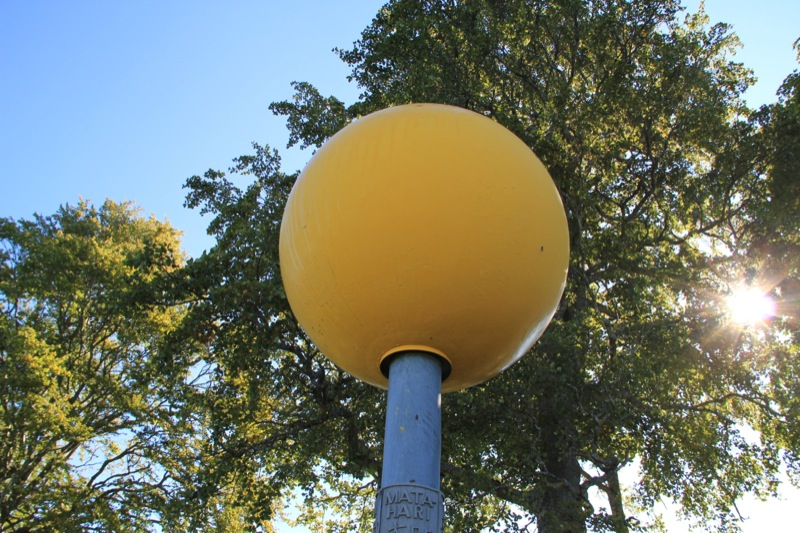
\includegraphics[width=0.318\textwidth]{pictures/sonne}
  \end{center}
%\caption{A gull}
\end{wrapfigure}
Häufig treten in alltäglichen oder wissenschaftlichen Kontexten, zum Beispiel in Physik, Biologie oder Chemie, grosse oder kleine Zahlen auf. Potenzen können dazu verwendet werden um sehr grosse oder sehr kleine Zahlen kurz und übersichtlich zu notieren. Zwei wichtige Beispiele für solche Zahlen sind folgend aufgeführt.

\begin{itemize}
\item Abstand Erde-Sonne, \definition{eine astronomische Einheit} (1 AE)
$$\unit[150'000'000]{km}$$
\item Durchmesser eines Atoms, \definition{ein \AA ngström} (1 \AA)
$$\unit[0.000\,000\,000\,1]{m}$$
\end{itemize}

\subsection{Der Potenzbegriff für natürliche Exponenten}
\begin{cdef}[Potenz, Basis und Exponent]
Seien $a\in\mathbb{R}_0^+$ und $n\in\mathbb{N}$. Der Term
$$a^b$$
heisst Potenz. $a$ nennt man Basis, $n$ heisst Exponent.
\end{cdef}

\begin{cdef}[Potenz mit natürlichem Exponenten]
Für $a\in\mathbb{R}_0^+$ und $n\in\mathbb{N}$ soll gelten:
$$a^1=a\quad\text{ und }\quad a^n=\underbrace{a\cdot a\cdot a\cdot\dots\cdot a}_{\text{n Faktoren}}\text{ für }n\geq2$$
\end{cdef}

\begin{uebenv}{natpot}
Berechne
    \begin{enumerate}[a)]
        \item $2^2$
        \item $2^3$
        \item $2^{10}$
        \item $3^3$
        \item $4^4$
        \item $5^3$
    \end{enumerate}
\end{uebenv}

\subsection{Zehnerpotenzen}
Nach Definition gilt also zum Beispiel
$$10^1=10\quad 10^2=100\quad 10^3=1000,$$
was leicht nachgerechnet werden kann. Die obige Liste weist auch ein System auf: Erhöht man nämlich den Exponenten einer Zehnerpotenz um $1$, so muss man einfach die entsprechende Zahl mit $10$ multiplizieren. Wenden wir dieses Prinzip rückwärts an, so können wir Bedeutungen für bislang sinnlose Ausdrücke
$$10^0\quad 10^{-1}\quad 10^{-2}\quad\text{etc.}$$
festlegen. Nämlich
$$10^0=1\quad10^{-1}=0.1=\frac{1}{10}\quad10^{-2}=0.01=\frac{1}{100}=\frac{1}{10^2}\quad\dots$$

Ich empfehle zu den jeweiligen Zehnerpotenzen auch die entsprechenden Präfixe und Ab\-kür\-zungen, vielleicht mit Tabelle \ref{tab:zehnerpotenzen} auf Seite \pageref{tab:zehnerpotenzen}, zu lernen. Sie gehören zu einer umfassenden Allgemeinbildung, da sie uns im Alltag begegnen.

\begin{table}
\begin{center}
\scalebox{0.85}{
  \begin{tabular}[ht]{lrlll}
  \rule[-3mm]{0mm}{24pt}
    $10^{15}\quad\quad$ & $1\,000\,000\,000\,000\,000$ & $\quad\quad\quad\quad\quad\quad1$ Billiarde & \hspace*{1cm}Peta- & P\\
    \rule[-3mm]{0mm}{24pt}
    $10^{12}\quad\quad$ & $1\,000\,000\,000\,000$ & $\quad\quad\quad\quad\quad\quad1$ Billion & \hspace*{1cm}Tera- & T\\
    \rule[-3mm]{0mm}{24pt}
    $10^{11}\quad\quad$ & $100\,000\,000\,000$ &  &  & \\
    \rule[-3mm]{0mm}{24pt}
    $10^{10}\quad\quad$ & $10\,000\,000\,000$ &  &  & \\
    \rule[-3mm]{0mm}{24pt}
    $10^{9}\quad\quad$ & $1\,000\,000\,000$ & $\quad\quad\quad\quad\quad\quad1$ Milliarde & \hspace*{1cm}Giga- & G\\
    \rule[-3mm]{0mm}{24pt}
    $10^{8}\quad\quad$ & $100\,000\,000$ &  &  & \\
    \rule[-3mm]{0mm}{24pt}
    $10^{7}\quad\quad$ & $10\,000\,000$ &  &  & \\
    \rule[-3mm]{0mm}{24pt}
    $10^{6}\quad\quad$ & $1\,000\,000$ & $\quad\quad\quad\quad\quad\quad1$ Million & \hspace*{1cm}Mega- & M\\
    \rule[-3mm]{0mm}{24pt}
    $10^{5}\quad\quad$ & $100\,000$ &  &  & \\
    \rule[-3mm]{0mm}{24pt}
    $10^{4}\quad\quad$ & $10\,000$ &  &  & \\
    \rule[-3mm]{0mm}{24pt}
    $10^{3}\quad\quad$ & $1\,000$ & $\quad\quad\quad\quad\quad\quad1$ Tausend & \hspace*{1cm}Kilo- & k\\
    \rule[-3mm]{0mm}{24pt}
    $10^{2}\quad\quad$ & $100$ &  & \hspace*{1cm}Hekto- & h\\
    \rule[-3mm]{0mm}{24pt}
    $10^{1}\quad\quad$ & $10$ &  & \hspace*{1cm}Deka- & d\\
    \rule[-3mm]{0mm}{24pt}
    $10^{0}\quad\quad$ & $1$ &  &  & \\
    \rule[-3mm]{0mm}{24pt}
    $10^{-1}\quad\quad$ & $0.1$ &  & \hspace*{1cm}Dezi- & d\\
    \rule[-3mm]{0mm}{24pt}
    $10^{-2}\quad\quad$ & $0.01$ &  & \hspace*{1cm}Centi- & c\\
    \rule[-3mm]{0mm}{24pt}
    $10^{-3}\quad\quad$ & $0.001$ & $\quad\quad\quad\quad\quad\quad1$ Tausendstel & \hspace*{1cm}Milli- & m\\
    \rule[-3mm]{0mm}{24pt}
    $10^{-4}\quad\quad$ & $0.000\,1$ &  &  & \\
    \rule[-3mm]{0mm}{24pt}
    $10^{-5}\quad\quad$ & $0.000\,01$ &  &  & \\
    \rule[-3mm]{0mm}{24pt}
    $10^{-6}\quad\quad$ & $0.000\,001$ & $\quad\quad\quad\quad\quad\quad1$ Millionstel & \hspace*{1cm}Mikro- & $\mu$\\
    \rule[-3mm]{0mm}{24pt}
    $10^{-7}\quad\quad$ & $0.000\,000\,1$ &  &  & \\
    \rule[-3mm]{0mm}{24pt}
    $10^{-8}\quad\quad$ & $0.000\,000\,01$ &  &  & \\
    \rule[-3mm]{0mm}{24pt}
    $10^{-9}\quad\quad$ & $0.000\,000\,001$ & $\quad\quad\quad\quad\quad\quad1$ Milliardstel & \hspace*{1cm}Nano- & n\\
    \rule[-3mm]{0mm}{24pt}
    $10^{-10}\quad\quad$ & $0.000\,000\,000\,1$ &  &  & \\
    \rule[-3mm]{0mm}{24pt}
    $10^{-11}\quad\quad$ & $0.000\,000\,000\,01$ &  &  & \\
    \rule[-3mm]{0mm}{24pt}
    $10^{-12}\quad\quad$ & $0.000\,000\,000\,001$ & $\quad\quad\quad\quad\quad\quad1$ Billionstel & \hspace*{1cm}Piko & p\\
    \rule[-3mm]{0mm}{24pt}
    $10^{-15}\quad\quad$ & $0.000\,000\,000\,000\,001$ & $\quad\quad\quad\quad\quad\quad1$ Billiardstel & \hspace*{1cm}Femto & f
  \end{tabular}
  }
    \end{center}
    \caption{Zehnerpotenzen: Namen und Abkürzungen}\label{tab:zehnerpotenzen}
 \end{table}

\subsection{Wissenschaftliche Darstellung}
Wir kommen auf unsere Motivation zu Beginn des Kapitels zurück; der schlanken Darstellung grosser und kleiner Zahlen. Bei der sogenannten \emph{wissenschaftlichen Darstellung} von Zahlen schreibt man die Zahl als Dezimalbruch mit Einer und Zehnerpotenzen.
\begin{bsp}
\ \\[-2ex]
\begin{itemize}
\item Abstand Erde-Sonne:
$$\unit[150'000'000]{km}=\unit[1.5\cdot10^8]{km}$$
\item Durchmesser eines Atoms:
$$\unit[0.000\,000\,000\,1]{m}=\unit[1\cdot10^{-10}]{m}$$
\item $$92'300=9.23\cdot10^4$$
\item $$0.0032=3.2\cdot10^{-3}$$
\end{itemize}
\end{bsp}

\begin{uebenv}{expand}
  Schreibe die Zahlen aus:

    \begin{enumerate}[a)]
      \item $2.52\cdot10^{5}$
      \item $6.52\cdot10^{7}$
      \item $5.555\cdot10^{12}$
      \item $4.15\cdot10^{9}$
      \item $4.31\cdot10^{9}$
      \item $3.11\cdot10^{3}$
      \item $1.23\cdot10^{6}$
      \item $6.22\cdot10^{4}$
    \end{enumerate}
\end{uebenv}

\begin{uebenv}{factor}
  Schreibe in wissenschaftlicher Darstellung:

    \begin{enumerate}[a)]
      \item $99'000'000$
      \item $4'180'000'000$
      \item $48'500'000$
      \item $0.000\,008\,21$
      \item $92'400$
      \item $0.000\,016$
      \item $190'300$
      \item $2'340$
      \item $1'350'000$
      \item $0.000\,000\,000\,101$
      \item $0.000\,000\,077$
    \end{enumerate}
\end{uebenv}

\subsection{Rechenregeln für Potenzen}

Mit der Definition einer Potenz lassen sich leicht die folgenden Gesetze einsehen.

Für die folgenden Ausführungen seien $a,b\in\mathbb{R}$ und $m,n\in\mathbb{N}$; sowie bei Bedarf $n>m$. Es gilt
\begin{align}
a^n\cdot a^m&=a^{n+m}\\
a^n\div a^m&=a^{n-m}\\
\left(a^n\right)^m&=a^{n\cdot m}\\
a^n\cdot b^n&=(a\cdot b)^{n}\\
a^n\div b^n&=(a\div b)^{n}
\end{align}

\begin{bsp}
Folgend je ein konkretes Beispiel:
\begin{itemize}
\item $x^{2n}\cdot x^{3-n}=x^{2n+3-n}=x^n+3$
\item $z^7\div z^{3-n}=z^{7-(3-n)}=z^{n+4}$
\item $\left(2^3\right)^4=2^{3\cdot4}=2^{12}=4096$
\item $2^4\cdot5^4=(2\cdot5)^4=10^4=10000$
\item $25^3\div5^3=(25\div5)^3=5^3=125$
\end{itemize}
\end{bsp}

\clearpage

\subsection{Notizen zu den Übungen}

\begin{lsg}{natpot}
        \begin{enumerate}[a)]
        \item $2^2=2\cdot2=4$
        \item $2^3=2\cdot2\cdot2=8$
        \item $2^{10}=1024$
        \item $3^3=27$
        \item $4^4=(2^2)^4=2^8=256$
        \item $5^3=125$
    \end{enumerate}
\end{lsg}
\begin{lsg}{expand}
        \begin{enumerate}[a)]
      \item $252\,000$
      \item $65\,200\,000$
      \item $5\,555\,000\,000\,000$
      \item $4\,150\,000\,000$
      \item $4\,310\,000\,000$
      \item $3110$
      \item $1\,230\,000$
      \item $62\,200$
    \end{enumerate}
\end{lsg}
\begin{lsg}{factor}
    \begin{enumerate}[a)]
      \item $9.9\cdot10^7$
      \item $4.18\cdot10^9$
      \item $4.85\cdot10^7$
      \item $8.21\cdot10^{-6}$
      \item $9.2400\cdot10^4$
      \item $1.6\cdot10^{-5}$
      \item $1.903\cdot10^5$
      \item $2.34\cdot10^3$
      \item $1.35\cdot10^6$
      \item $1.01\cdot10^{-10}$
      \item $7.7\cdot10^{-8}$
    \end{enumerate}
\end{lsg}

\clearpage

\section{Zahlensysteme}

\subsection{Eine kurze Geschichte der Zahlen}

\begin{wrapfigure}{r}{0.382\textwidth}
  \begin{center}
    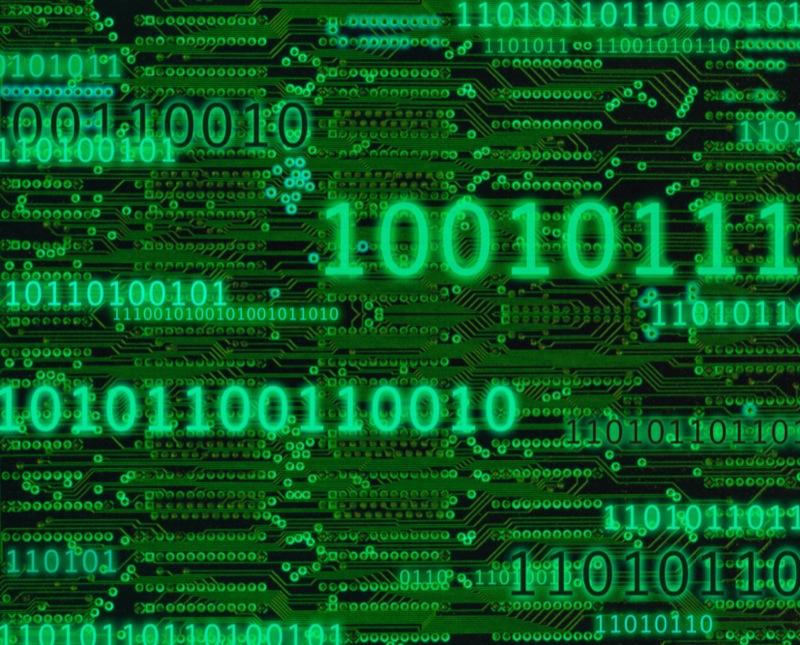
\includegraphics[width=0.382\textwidth]{pictures/binary}
  \end{center}

\end{wrapfigure}
Es ist nicht genau bekannt, seit wann die Menschen Zahlen benutzen. Die ersten Darstellungen von Zahlen waren wahrscheinlich Striche. Man spricht hier von einem unären Zahlensystem, weil alle Zahlen mit nur einem Zeichen (Strich) dargestellt werden.

\begin{uebenv}{fnfstriche}
Weshalb fasst man just fünf Striche zu einem Bündel zusammen?
\end{uebenv}

\subsection{Zahlen in Babylonien (ca. 2000 v. Chr.)}
\begin{figure}[h]
\begin{center}
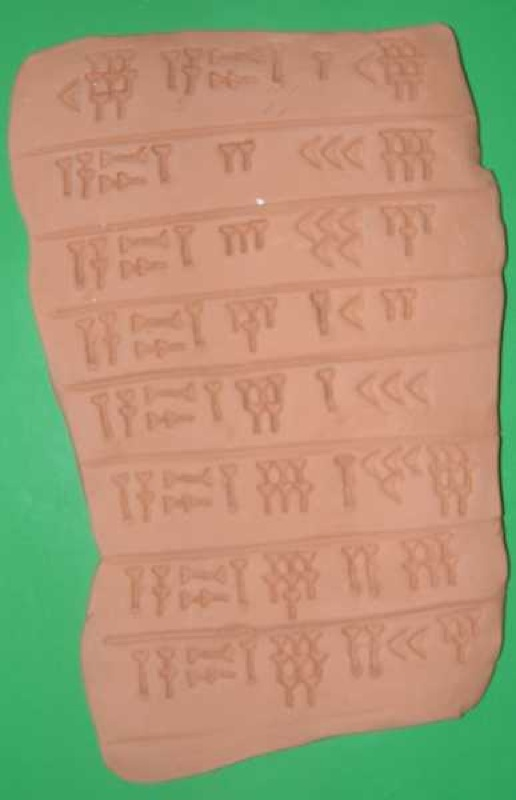
\includegraphics[width=0.35\textwidth]{pictures/babylontafel}\hspace*{0.2cm}
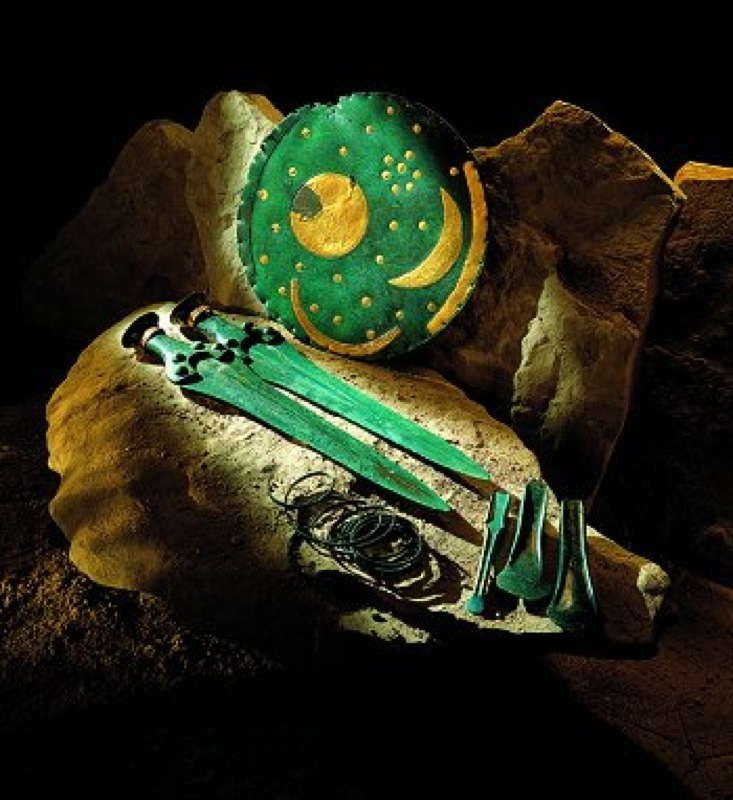
\includegraphics[width=0.35\textwidth]{pictures/babylonuhr}
\end{center}
\caption{Babylonische Rechentafel und Sternkarte}
\end{figure}
Die Babylonier verwendeten als eines der ersten Völker ein sogenanntes \definition{Positionssystem}. Der Wert eines Zeichens hängt auch von dessen Position ab. Während wir heute in unserem Dezimalsystem (Basis 10) die Ziffern $0, 1, 2, \dots, 9$ verwenden, brauchten die Babylonier in ihrem Sechzigersystem $59$ Ziffern, denn ein Zeichen für die Null gab es damals noch nicht.

Abschliessend noch ein Beispiel, wie diese Zeichen verwendet werden.
\begin{center}
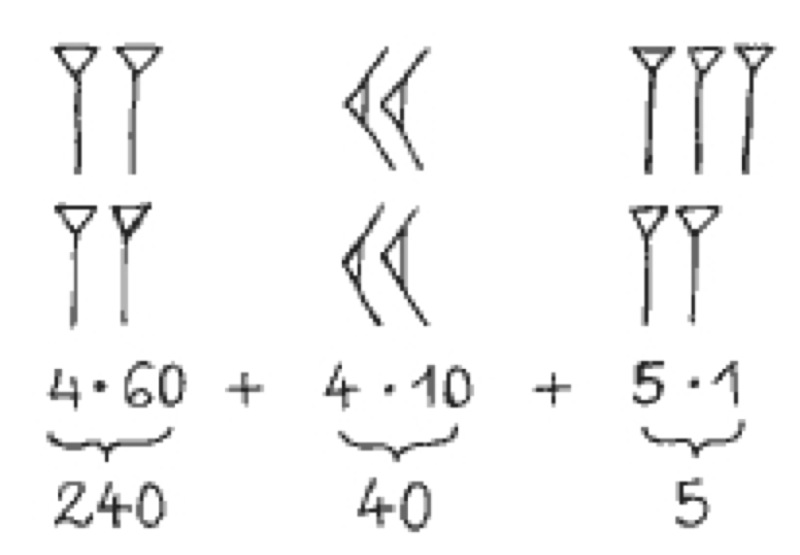
\includegraphics[width=5cm]{pictures/babylon285}
\end{center}

\subsection{Zahlen in Indien und Arabien}

Die Ziffern, wie wir sie heute verwenden, haben ihren Ursprung in Indien und Arabien. Sie wurden unter anderem durch Kaufleute wie Fibonacci im 13. Jahrhundert nach Europa gebracht, konnten sich aber erst später gegen die römischen Zahlen durchsetzen.

Eine grossartige Leistung des menschlichen Geistes stellt die Erfindung der Zahl Null dar. Für die Menschen war es lange Zeit unvorstellbar, ein Zeichen für \glqq Nichts\grqq\  zu gebrauchen. Bei Positionssystemen ist ein Zeichen für Null als Platzhalter aber unentbehrlich.

\begin{figure}[h]
\begin{center}
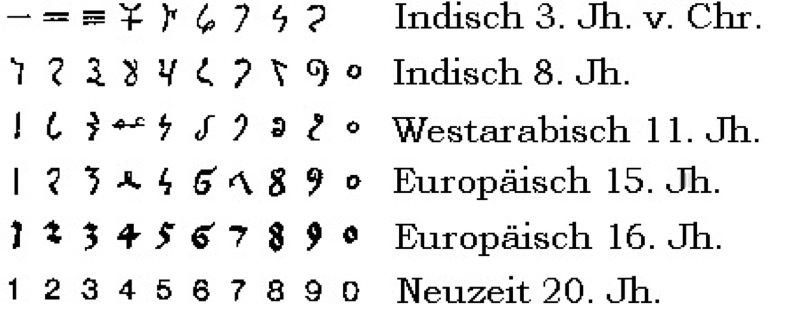
\includegraphics[width=0.7\textwidth]{pictures/entwzahl}
\end{center}
\caption{Evolution von den indischen bis zu den heutigen arabischen Ziffern}
\end{figure}

\begin{uebenv}{rmisch}
Lerne die römischen Zahlen von $1$ bis $3000$.
\end{uebenv}

\begin{uebenv}{jahreszahl}
Schreibe $\the\year$ mit römischen Zahlzeichen; und $1848$.
\end{uebenv}

\begin{figure}
\begin{center}
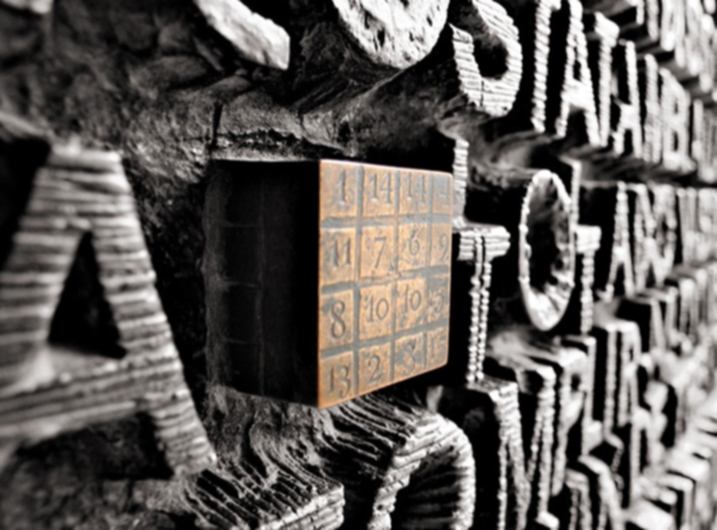
\includegraphics[width=0.618\textwidth]{pictures/magquadr}
\end{center}
\caption{Magisches Quadrat am Tor der Familia Sagrada}
\end{figure}

\subsection{Zahlensysteme}

Ein Zahlensystem wird zur Darstellung von Zahlen verwendet. Eine Zahl wird dabei nach den Regeln des Zahlensystems als Folge von Ziffern dargestellt. Man unterscheidet im Wesentlichen zwischen Additionssystemen und Stellenwertsystemen (Positionssystemen).

Ein \definition{Positionssystem} hat eine Basis $b\in\mathbb{N}\setminus\{1\}$. Jede Zifferposition hat einen Wert, der einer Potenz der Basis entspricht. Für die $k$-te Position, $k\in\mathbb{N}_0$ hat man einen Wert von $b^{k-1}$.
Die Berechnung des Zahlenwertes erfolgt durch Multiplikation der einzelnen Ziffern $z_i$ mit den zugehörigen Stellenwerten $b_i$ und Summation dieser Produkte:
$$\text{Zahlenwert} = z_n\cdot b^n+\dots+z_i\cdot b^i+\dots+z_0\cdot b^0.$$
\begin{bsp}
Unter
\marginnote{
<<<<<<< Updated upstream
\qrcode{
https://www.youtube.com/watch?v=j3uGEq0mXIk}
=======
\href{https://www.youtube.com/watch?v=j3uGEq0mXIk}{\qrcode{https://www.youtube.com/watch?v=j3uGEq0mXIk}}
>>>>>>> Stashed changes
}
der Zahl $1257$ im üblichen Dezimalsystem (d.h. die Basis ist $10$) verstehen wir den Wert
$$1\cdot10^3+2\cdot10^2+5\cdot10^1+7\cdot10^0 = 1257.$$
\end{bsp}

Mit der Beschränkung des niedrigsten Exponenten auf $0$ kann man nur ganze Zahlen darstellen. Lässt man auch negative Exponenten zu, kann man auch rationale Zahlen in einem Stellenwertsystem schreiben, wobei der Übergang vom nichtnegativen zum negativen Exponenten durch ein Trennzeichen markiert wird, beispielsweise einen Punkt:
$$1\cdot10^2+2\cdot10^1+1\cdot10^0+4\cdot10^{-1}+7\cdot10^{-2}=121.47$$

\begin{uebenv}{binr}
Computer stellen Zahlen nur mit den Ziffern $0$ und $1$ dar und zwar als magnetische Polung oder elektrisches Signal (Nord oder Süd bzw. Plus oder Minus).
Die binäre Zahl $1011$ entspricht der Dezimalzahl
$$1\cdot2^3+0\cdot2^2+1\cdot2^1+1\cdot2^0=8+2+1=11.$$
Stelle die Dezimalzahlen von $1$ bis $20$ im Binärsystem dar.
\end{uebenv}

\begin{uebenv}{decbin}
Finde für die Dezimalzahlen $34$ und $37$ die Binärschreibweise.
\end{uebenv}

\begin{uebenv}{pibin}
    Stelle die Zahl $\pi$ binär mit sechs Nachkommastellen dar.
\end{uebenv}

\subsection{Das Sexagesimalsystem}

Das babylonische Zahlensystem ist ein Stellenwertsystem zur Basis 60, mit dem beliebig grosse, aber auch beliebig kleine Zahlen systematisch dargestellt werden können. Die Babylonier benutzten eine Keilschrift. Hier sind die ersten 59 Zahlen.

\begin{figure}[h]
\begin{center}
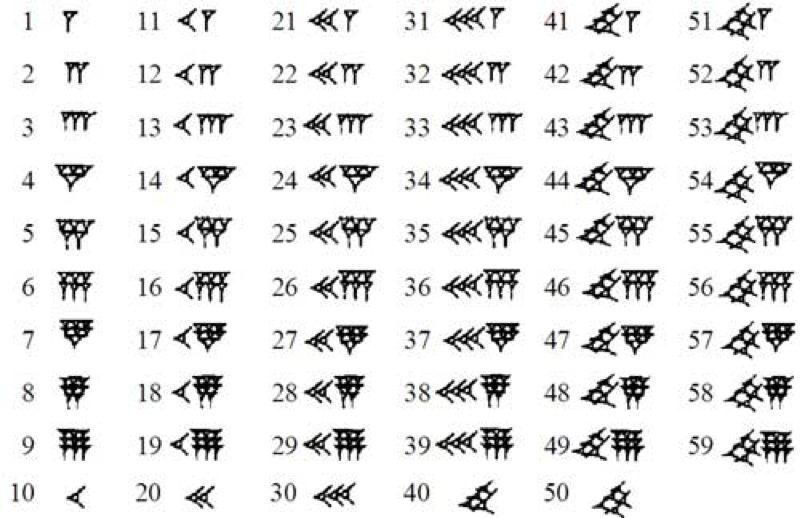
\includegraphics[width=0.7\textwidth]{pictures/babylonzahlen}
\end{center}
\caption{Babylonische Zahlen von 1 bis 59}
\end{figure}

Jede dieser oben aufgeführten Zahlen ist als eine Ziffer zu interpretieren. Erst bei Zahlen über $59$ wird naturgemäss die nächste Stelle benutzt. Sie wird, wie auch bei unserem Dezimalsystem, nach links eingerückt.

\begin{center}
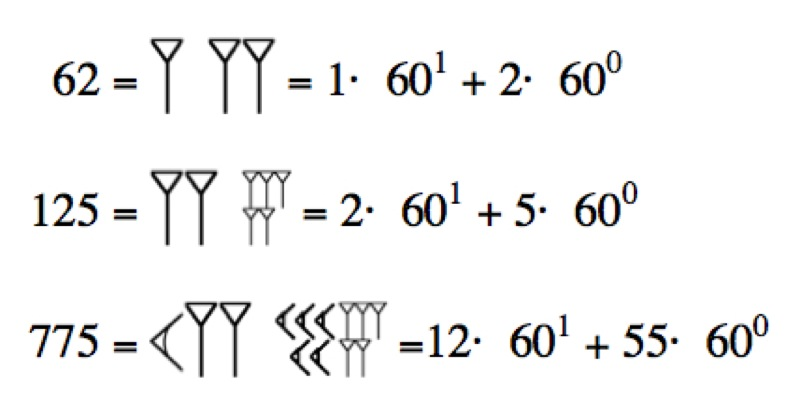
\includegraphics[width=0.5\textwidth]{pictures/babylongrossezahlen}
\end{center}
Genauso interessant ist, dass die Babylonier ihr Stellenwertsystem auch für Nachkommazahlen nutzten. Dabei kam ihnen die vielfältige Teilbarkeit der Zahl 60 zugute --- dies war vermutlich auch der Grund, weshalb das Sexagesimalsystem überhaupt eingeführt wurde. Ein Zeichen für den \glqq Punkt\grqq\ war nicht vorhanden, so dass die Zuordnung der Stellen zu den $60$-er Potenzen nicht eindeutig war. Welche Position z.B. die $60^0$-Stelle hat, musste aus dem Kontext erraten werden.
\begin{center}
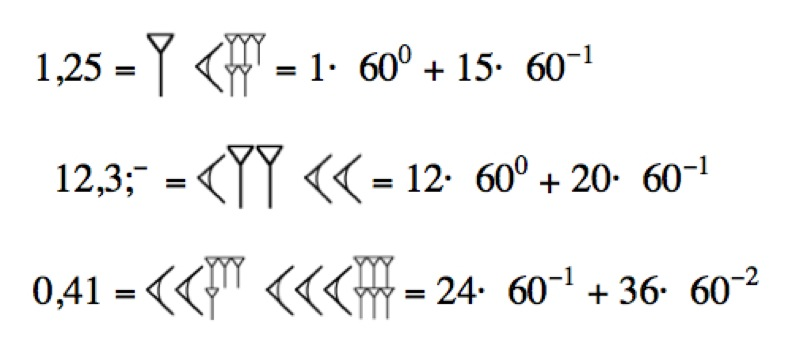
\includegraphics[width=0.4\textwidth]{pictures/babylonnachkomma}
\end{center}

\begin{figure}
\begin{center}
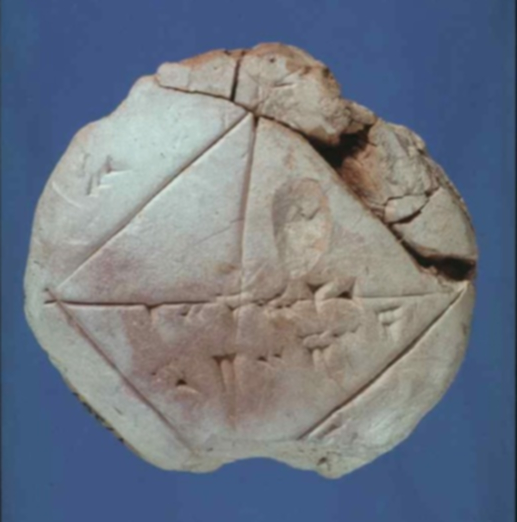
\includegraphics[width=0.45\textwidth]{pictures/tontafel}
\end{center}
\caption{Babylonische Tontafel, 7289 v.Chr.}\label{abb:tontafel}
\end{figure}

Eine genaue Untersuchung des Objekts aus Abbildung \ref{abb:tontafel} auf Seite \pageref{abb:tontafel} fördert folgendes Schriftbild zu Tage, das in Abbildung \ref{interpretation} auf Seite \pageref{interpretation} deutlicher zu erkennen ist. Es zeigt sich, dass man ein sinnvolles Ergebnis kriegt, wenn man die erste \glqq1\grqq\ mit $1\cdot60^0$ identifiziert. Wir erhalten so für die erste Zeile
$$1\cdot60^0+24\cdot60^{-1}+51\cdot60^{-2}+10\cdot60^{-3}$$

\begin{uebenv}{irrational}
Welche Zahl wird hier beschrieben?
\end{uebenv}

\begin{figure}
\begin{center}
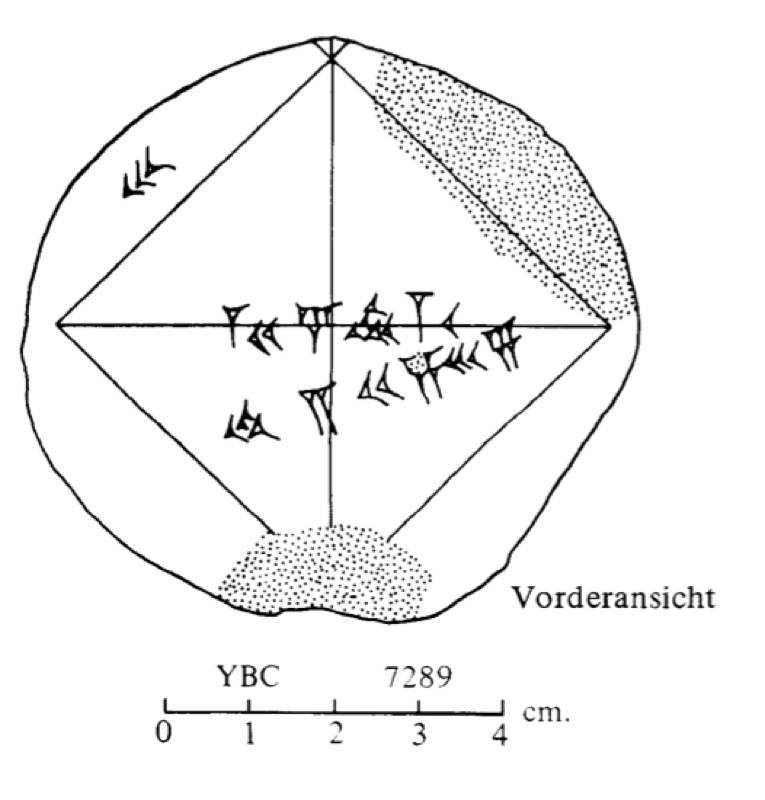
\includegraphics[width=0.35\textwidth]{pictures/tontafelschema}
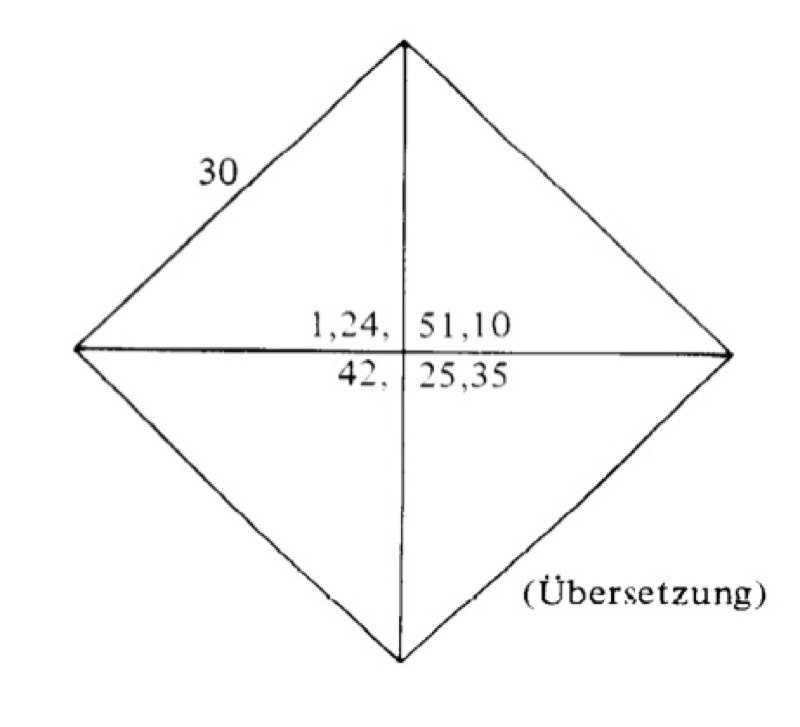
\includegraphics[width=0.35\textwidth]{pictures/schema}
\end{center}
\caption{Schema und Übersetzung der Zahlen}\label{interpretation}
\end{figure}

\begin{landscape}
\begin{figure}[h]
\begin{center}
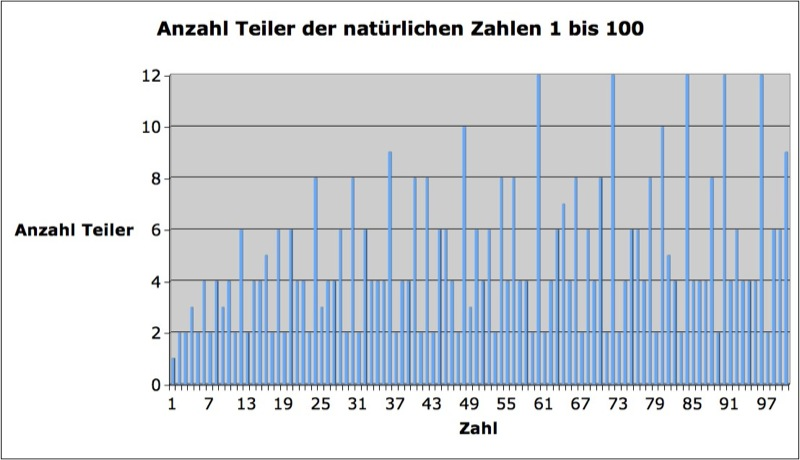
\includegraphics[height=0.7\textheight]{pictures/anzahlteiler}
\end{center}
\caption{Anzahl Teiler der ersten hundert natürlichen Zahlen}
\end{figure}
\end{landscape}

\clearpage

\subsection{Notizen zu den Übungen}

\begin{lsg}{fnfstriche}
Vermutlich kommt dies vom Zählen mit den Fingern.
\end{lsg}

\begin{lsg}{rmisch}
Von \texttt{I} bis \texttt{M} kann man diese Ziffern kombinieren. Beachte, dass nie mehr als drei gleichartige Ziffern nebeneinander stehen. Steht aber eine minderwertige Ziffer links einer höherwertigen, so wird ihr Wert abgezogen.
\end{lsg}

\begin{lsg}{jahreszahl}
\texttt{MMXXIV} und \texttt{MDCCCXLVIII}
\end{lsg}

\begin{lsg}{binr}
\begin{tabular}{|c|c|c|c|}
  \hline
  \textbf{BIN} & \textbf{DEC} & \textbf{BIN} & \textbf{DEC} \\
  \hline
  0001 & 1 & 1011 & 11 \\
  0010 & 2 & 1100 & 12 \\
  0011 & 3 & 1101 & 13 \\
  0100 & 4 & 1110 & 14 \\
  0101 & 5 & 1111 & 15 \\
  0110 & 6 & 10000 & 16 \\
  0111 & 7 & 10001 & 17 \\
  1000 & 8 & 10010 & 18 \\
  1001 & 9 & 10011 & 19 \\
  1010 & 10 & 10100 & 20 \\
  \hline
\end{tabular}
\end{lsg}

\begin{lsg}{decbin}
$34=1\cdot2^5+1\cdot2^1=100010_{(2)}$ und $37=1\cdot2^5+1\cdot2^2+1\cdot2^0=100101_{(2)}$
\end{lsg}

\begin{lsg}{pibin}
    $3=11_{(2)}$ und weiter haben $2^{-3}$ und $2^{-6}$ Platz: $11.001001\dots$
\end{lsg}

\begin{lsg}{irrational}
Es ist $1\cdot60^0+24\cdot60^{-1}+51\cdot60^{-2}+10\cdot60^{-3}=1.41421\overline{296}$, was nahe bei $\sqrt{2}=1.414213\dots$ ist.
\end{lsg}

\cleardoublepage

\listoffigures

\end{document}